\chapter{Main results}
\label{chapter:estimates}

%--------------------------------------------------------------------------------------%
This chapter is devoted to the main theoretical and numerical findings obtained during 
the PhD studies. Along the exposition of the results, we refer to the published works
\cite{RefMatculevichNeittaanmakiRepin2013, RefMatculevichRepin2014, 
RefMatculevichNeitaanmakiRepin2015, RefMatculevichRepinPoincare2014} and preprint 
\cite{RefArxivMatculevichRepin2015}, where corresponding matters are thoroughly 
discussed. 

\section{Fully reliable Adaptive Picard--Lindel\"{o}f method}
\label{sec:pl-guaranteed-method}

In this section, we make an overview of the work dedicated to the fully reliable APL 
method which was suggested in \cite{RefMatculevichNeittaanmakiRepin2013} in order to 
reliably solve the Cauchy problem. The details of the study can also be found in 
\cite[Section 6.7.6]{Malietall2014}. 

%--------------------------------------------------------------------------------------%
Let $Q := \big\{(u,\;t)\;\vert\;u \in \mathrm{U},\; t \in I \big\}$, where $\mathrm{U}$ 
is the set of possible values of $u$ determined during an a priori analysis of the 
problem and $I := [t_0, t_K]$. We consider the problem \eqref{eq:cauchy-problem} from 
Section \ref{ssec:pl-method} and assume that function $\varphi(u(t),\:t)$ is continuous 
with respect to both variables and satisfies the Lipschitz condition for any 
$(u_1,\;t_1)$, $(u_2,\;t_2)\:\in Q$ in the form
%
\begin{equation*}
	\|\varphi(u_2,\;t_2) - \varphi(u_1,\;t_1)\|_{C([t_1,\;t_2])} \leq
	\constL_1 \|u_2 - u_1\|_{C([t_1,\;t_2])} + \constL_2 \vert t_2 - t_1 \vert,
	\label{eq:iter3-lipschitz-property}
\end{equation*}
%
where $\constL_1$ and $\constL_2$ are Lipschitz constants.

%--------------------------------------------------------------------------------------%
Assume that $I$ is discretized in the following way:
%
\begin{equation}
I = \cup_{ I^{(k)} \subset \mathcal{F}_K } \overline{I^{(k)}}, \quad 
\mathcal{F}_K := \{I^{(k)}\}_{k = 0}^{K-1}, 
\quad I^{(k)} := (t_k,\;t_{k+1}), 
\quad K \in \Nd.
\label{eq:F-K}  
\end{equation}
%
If we consider \eqref{eq:iterative-form-of-problem}, it becomes clear that condition 
%--------------------------------------------------------------------------------------%
$q := \constL_1(t_{k+1} - t_k) < 1$
%
provides the convergence of the algorithm by adapting the length of interval \linebreak
$I^{(k)} \subset \mathcal{F}_K$ to constant $\constL_1$. Thus, if $I^{(k)}$ is 
sufficiently small, the solution can be reconstructed by an iteration scheme, which we 
call an Adaptive \PL \linebreak(APL) method. The corresponding errors of the iterative 
approximations can be controlled by the Ostrowski estimates
%
\begin{equation*}
	\mij{j} := \tfrac{1}{1+q} \|u_j - u_{j + 1}\|_{C(I^{(k)})} \leq \|u - u_j\|_{C(I^{(k)})}
	\leq \tfrac{q}{1-q} \|u_j - u_{j - 1}\|_{C(I^{(k)})} =: \maj{j}.
	%\label{eq:iter3-ostrowski-upper-bound}
\end{equation*}
%
The latter one is applicable to any iterative process with a contraction operator
that possesses the computable contractivity parameter, for example to the iteration 
algorithm provided in work \cite{GiraultKumarWheeler2015}.

%--------------------------------------------------------------------------------------%
However, some technical difficulties arising in iterative integration must be dealt 
with. Consider $I^{(k)} \in \mathcal{F}_K$ introduced in \eqref{eq:F-K} and assume that 
the initial guess $u_0$ is defined as a piecewise affine function on a sub-mesh 
$\Omega_{S_k}$ of $I^{(k)}$, i.e., \linebreak 
$\Omega_{S_k} = \cup_{s = 0}^{S_k \minus 1}[z_s, z_{s + 1}]$, where 
$\Delta_s = z_{s + 1} - z_s$, $z_0 = t_k$, and $z_{S_k} = t_{k+1}$. As the first 
sub-interval, we have
%
\begin{equation}
  u_1(t) = \Int_{t_0}^{t} \varphi(u_0(s),\;s) \ds+a_0,\quad t \in I^{(0)} := [t_0, t_1].
  \label{eq:first-step}
\end{equation}
%
If $q < 1$, the distance between the computed $u_1$ and $u$ can be found by means of 
%
\begin{equation}
   \|u_1(t) - u(t)\|_{C(I^{(0)})} \leq \tfrac{q}{1-q} \|u_1(t) - u_0(t)\|_{C(I^{(0)})}.
	\label{eq:ostrowski-upper-bound-on-first-step}
\end{equation}
%
%--------------------------------------------------------------------------------------%
However, in \eqref{eq:first-step} we obtain piecewise polynomials as a result of the 
integration of piecewise affine functions. 
%
\begin{figure}[th]
\begin{center}
	\input{pics/integration}
	\caption{Integration and interpolation errors generated by $\Tau$.}
	\label{fig:integration-process}
\end{center}
\end{figure}
%
In order to perform iterations on a finite dimensional space $X_h$, the additional 
errors caused by integration and mapping of a function to this finite dimensional space 
must be taken into account (see Figure \ref{fig:integration-process}).
%
Due to the numerical representation of $\Tau$, i.e., $\Tau_h:\; X_h \rightarrow Z_h$, 
where $Z_h \subset X$, the function $\widehat{x}_j = \Tau_h x_{j-1}$ contains an 
integration error. Since $Z_h \subset X$ does not coincide with $X_h$, we must apply a 
certain projection (interpolation) operator $\uppi$ and evaluate the corresponding 
error. 
%
%--------------------------------------------------------------------------------------%
Henceforth, the errors generated by numerical integration appear in
(\ref{eq:ostrowski-upper-bound-on-first-step}) as follows:
%
\begin{equation}
      \|u_1 - u_0\|_{C(I^{(0)})} \leq
            \:\|u_0 - \widehat{u}_1\|_{C(I^{(0)})}
						+ \|\widehat{u}_1 - u_1\|_{C(I^{(0)})}.
 \label{eq:estimate-included-integration-error}
\end{equation}
%
Here, $\|\widehat{u}_1 - u_1\|_{C(I^{(0)})} := \|\widehat{e}_1\|_{C(I^{(0)})}$ is the 
{\em integration error}. Then we must project the result of numerical integration 
$\widehat{u}_1 \in Z_h$ to $X_h$, i.e., 
%
$    \overline{u}_1(t) = \uppi \, \widehat{u}_1\:\in CP^1(I^{(0)})$,
%
where $\uppi: Z_h \rightarrow CP^1(I^{(0)})$ is the projection operator such that 
$\uppi \widehat{u}(z_s) = \overline{u}(z_s)$, $s = 0, \ldots, S_k \minus 1$. Thus, the RHS 
of (\ref{eq:estimate-included-integration-error}) is modified as follows
%--------------------------------------------------------------------------------------%
%
\begin{equation*}
    \|u_1 - u_0\|_{C(I^{(0)})} \leq
		\:\|\overline{u}_1 - u_0\|_{C(I^{(0)})}
		+ \|\widehat{u}_1 - u_1\|_{C(I^{(0)})}
		+ \|\widehat{u}_1 - \overline{u}_1\|_{C(I^{(0)})}	,
    %\label{eq:estimate-included-interpolation-error}
\end{equation*}
%
Here, 
$\|\widehat{u}_1(t) - \overline{u}_1(t)\|_{C(I^{(0)})} =: \|\overline{e}_1\|_{C(I^{(0)})}$ 
is the {\em interpolation error}. 

%--------------------------------------------------------------------------------------%
The obtained result states that for any piecewise linear approximation \linebreak 
$v(t) := v^k(t)$, $t \in I^{(k)}$, and exact solution $u(t)$ the following estimate
%
$$\| u(t) - v(t) \|_{C(I^{(k)})} \leq \M^{k}, \quad t \in I^{(k)}, \quad
I^{(k)} \subset \mathcal{F}_K,$$
%
holds. Here, the piecewise constant error bound reads as
%
$$\M^{k} := \tfrac{q}{1-q} 
(\|\overline{v}_{j+1} - \overline{v}_{j}\|_{C(I^{(k)})} + e^{\rm int}_{j} + e^{\rm interp}_{j}).$$ 
%
where 
%
\begin{equation}
  e^{\rm int}_j := \Sum_{s = 0, ..., S_k - 1} 
		\bigg(\tfrac{\mathrm{\constL_s}}{2} \Delta_s^2 -
    \tfrac{1}{2\mathrm{\constL_s}} \Big[\varphi(\overline{v}_{j,\:s+1}, z_{s+1}) -
    \varphi(\overline{v}_{j,\:s}, z_s)\Big]^2\bigg),
  \label{eq:iter3-general-integration-estimate}
\end{equation}
%
and 
%
\begin{multline}
  e^{\rm interp}_j \! := \! \! \! \! \Sum_{s = 0, ..., S_k - 1} 
	\! \! \Delta_s \bigg(\tfrac{1}{8} \big(\varphi(\overline{v}_{j,\:s+1}, z_{s+1})
    - \varphi(\overline{v}_{j,\:s}, z_s)\big) \\
		+ \tfrac{2}{3} \Big[ \constL_{1,\;s}
    \vert \overline{v}_{j,\;s+1} - \overline{v}_{j,\;s} \vert +
      \constL_{2,\;s} \Delta_s \;\Big] \bigg)
  \label{eq:iter3-general-interpolation-estimate}
\end{multline}
%
%--------------------------------------------------------------------------------------%
are integration and interpolation estimates of $\|\widehat{e}_j\|_{C(I^{(k)})}$ and
$\|\overline{e}_j\|_{C(I^{(k)})}$ on the $j^{\rm th}$ iteration. Constants in 
\eqref{eq:iter3-general-integration-estimate} and 
\eqref{eq:iter3-general-interpolation-estimate} are 
$\constL_s = \constL_{1,\;s}\:l_s + \constL_{2,\;s}$, where $l_s$ is the 
slope of a piecewise function on every interval $[z_s,\;z_{s+1}]$, $s = 0, ... ,S_k 
\minus 1$, 
and local Lipschitz constant $\constL_{1,\;s}$ analogous to the one in 
\eqref{eq:iter3-lipschitz-property}. In \cite{RefMatculevichNeittaanmakiRepin2013} and 
\cite[Section 6.7.6]{Malietall2014}, we present detailed derivation of 
estimates for both errors, and confirm the theoretical findings by set of numerical 
examples.

%-------------------------------------------------------------------------------------%
\section{Guaranteed error estimates for the solution of parabolic I-BVPs}
\label{sec:guaranteed-parabolic-equation}
%-------------------------------------------------------------------------------------%

This section presents two forms of the functional error estimates, which provide a 
guaranteed upper bound of the deviation $e = u - v$ for the generalized solution $u$ 
of I-BVP (\ref{eq:generalized-statement}) with $a \equiv 0$ and any function 
$v \in \HD{1, 1}{0}(Q_T)$ (generated for instance by some numerical method) measured 
in terms of the norm
%
\begin{multline}
	\error_{(\nu, \theta, \zeta, \chi)}
	:= \! \Int_0^T \big( \nu \left \| \, \nabla e \, \right\|^2_{A} \,
	%+ \, \theta \left\| \, \varrho \, e \right\|^2_\Omega \, 
	+ \, \theta \left\| \, \lambda \, e \right\|^2_\Omega \, 
	+ \, \chi \! \left\| \, \sigma\, e \, \right\|^2_{\Gamma_R}  \big) \dt
	+ \, \zeta \! \, \left \| \, e (\cdot, T) \, \right \|^2_{\Omega},	
	\label{eq:energy-norm}
\end{multline}
%
where $\nu$, $\theta$, $\zeta$, $\chi$ are positive weights and 
%
%\begin{equation*}
%$\varrho_0^2 \leq \varrho^2 := \lambda^2$
% - \tfrac{1}{2} \, \dvrg \,a$
%$\varrho_0^2 \leq \varrho^2 := \lambda^2$, $a \eq 0$,
%\end{equation*}
%
function %$a$ and 
$\lambda$ satisfies (\ref{eq:coefficients-condition}). 
%In case $a \neq 0$, the idea of 
%the method is practically the same, however we omit 
%it if frames of this work to simplify
%the exposition. 
%
%-------------------------------------------------------------------------------------%
By selecting the weights to balance the components in (\ref{eq:energy-norm}) with a 
desired proportion, we generate a collection of error measures, which can be used for \
judging the distance between $u$ and $v$.

%--------------------------------------------------------------------------------------%
The first form of the majorant is presented and numerically tested for evolutionary 
reaction-diffusion I-BVPs of parabolic type in \cite{RefMatculevichRepin2014}. 
%--------------------------------------------------------------------------------------%
The second (advanced) form of the majorant is studied in 
\cite{RefMatculevichNeitaanmakiRepin2015} and \cite{RefMatculevichRepinPoincare2014}. 
Latter one was introduced originally in publication of Repin \cite{Repin2002} in order 
to improve the recovery of the error in balance equation \eqref{eq:parabolic-equation} 
by using a special correction function $w$ (see 
Theorem \ref{th:theorem-minimum-of-majorant-II}).
In \cite{RefMatculevichNeitaanmakiRepin2015}, we extend both majorants for problems 
formulated on domains of complicated geometry by suggesting a method of decomposition 
of $\Omega$ and application of the Poincar\'{e} inequalities locally to each element
from the collection of subsets. 
%
This method does not only help to overcome the complications caused by estimating the 
global Friedrichs constant but also improves the efficiency of the resulting estimates 
which exploit the constant on the smaller sub-domains. 
In \cite{RefMatculevichRepinPoincare2014}, we encounter difficulties caused by the
mixed BC with a non-trivial input function and overcome them by exploiting the 
Poincar\'{e}-type inequalities. The obtained estimates become fully guaranteed, due 
to results of \cite{NazarovRepin2014} and \cite{RefArxivMatculevichRepin2015}, where 
reliable and easy computable bounds for the constants in the Poincar\'{e}-type 
inequalities are presented for simpleces in $\Rtwo$ and $\Rthree$ (commonly used in FE 
analysis).

%--------------------------------------------------------------------------------------%
The initial step in the derivation of both upper estimates is the transformation of 
\eqref{eq:generalized-statement} into the integral identity
%
\begin{multline}
	\Int_0^T \Big( 
	\left \| \, \nabla e \, \right\|^2_{A} \, + \,
	%\left\| \, \varrho \, e \right\|^2_\Omega \dt \, + \,
	\left\| \, \lambda \, e \right\|^2_\Omega \dt \, + \,
	\left\| \, \sigma\, e \, \right\|^2_{\Gamma_R} \Big) \dt \, + 
	\tfrac{1}{2} \! \, \left \| \, e (\cdot, T) \, \right \|^2_{\Omega} \, \\[-10pt]
	= \Int_{Q_T} \!\! \left( \big(f - v_t - \lambda^2 \, v %- a \cdot \nabla{v} 
	                         \big) \, e 
	                         - A \nabla{v} \cdot \nabla e \right) \dxt 
	+ \,\Int_{S_R} - \sigma^2 v \, e {\mathrm{\:d}s\mathrm{d}t},
	\label{eq:energy-balance-equation}
\end{multline}
%
which follows from the main energy-balance relation of problem 
(\ref{eq:parabolic-equation})--(\ref{eq:parabolic-robin-bc}).
It is worth mentioning that evolutionary I-BVPs, unlike elliptic BVPs, do not possess 
variational formulation, therefore the functional error estimates can only be obtained
from generalized identity (\ref{eq:generalized-statement}).   
%--------------------------------------------------------------------------------------%
Next, we rearrange the RHS of (\ref{eq:energy-balance-equation}) by introducing a `free' 
vector-valued function 
%
\begin{alignat*}{2}
	y \in Y_{\dvrg}(Q_T) := 
	\Big \{  y \in \L{2} \big(0, T; \L{2}\big(\Omega, \Rd\big)\big)\;\big|\; 
	& \dvrg y \in \L{2} \big(0, T; \L{2}(\Omega)\big), \; \nonumber\\[-9pt]
	& y \cdot n \in \L{2} \big(0, T; \L{2}(\Gamma_R)\big) \Big \}.
	%\label{eq:y-set-div}
\end{alignat*} 	
%
%--------------------------------------------------------------------------------------%
The {\em residuals} of (\ref{eq:parabolic-equation}), (\ref{eq:dual-part}),  
and (\ref{eq:parabolic-robin-bc}) are denoted by
%
\begin{alignat}{2}
	\R_{f}  (v, y) & := f - v_t - \lambda^2 \, v 
	%- a \cdot \nabla{v} 
	+ \dvrg \: y, \label{eq:r-f}\\[-3pt]
	\R_A  (v, y) & := y - A \nabla{v}, \label{eq:r-d} \\[-3pt]
	\R_{\sigma}  (v, y) & := -\sigma^2 v - y \cdot n, \label{eq:r-b}
\end{alignat}
%
respectively. Moreover, we define the weighted residuals
%
\begin{alignat}{2}
	\R_{f}^{\mu} (v, y) & := \mu \, \R_{f} \quad{\rm and} \quad
	\R_{f}^{1 \minus \mu}  (v, y) := (1 - \mu) \, \R_{f},
	\label{eq:r-mu}
\end{alignat}
%
%--------------------------------------------------------------------------------------%
where $\mu(x,t)$ is a real-valued function taking values in $[0, 1]$ used in order to 
split the residual with $\lambda$ into two parts. This way, the resulting estimate 
becomes robust to cases in which $\lambda$ attains drastically different values and may 
be close to zero in different parts of $\Omega$. A detailed numerical analysis of the 
majorant with the balancing parameter $\mu$ can be found in 
\cite[Sections 2, 5]{RefMatculevichRepin2014}.
%
The forthcoming summary demonstrates that a certain weighted combination of norms of
\linebreak 
\eqref{eq:r-f}--\eqref{eq:r-mu} controls the distance between $u$ and $v$. 

%--------------------------------------------------------------------------------------%
\begin{theorem}
\label{th:theorem-minimum-of-majorant-I}
%
For any $v \in \VD{1, 1}{0}(Q_T)$, $y \in Y_{\mathrm{div} \:}(Q_T)$, $\delta \in (0, 2]$, 
and real-valued function $\gamma(t) \in \big[\tfrac12, +\infty\big[$, we have the 
estimate
%
\begin{multline}
	\error_{({\nu},\, {\theta},\, 1, \,2)}
	\leq \majone (v, y; \delta, \gamma, \mu) \!
	:= \| e (\cdot, 0) \|^2_{\Omega} \,
	+ \, \Int_0^T \! \! \Big ( 
	\, \gamma(t) \left\|\,\tfrac{1}{\lambda}\,\R_{f}^{\mu}\,\right\|^2_{\Omega} \,\\[-7pt]
	+ \alpha_1 \|\,\R_A \,\|^2_{A^{\minus 1}} 
	+ \, \alpha_2 \,\tfrac{\CFriedrichs^2}{\,\underline{\nu}_A}
		\left\| \, \R_{f}^{1 \minus \mu} \, \right \|^2_{\Omega} \,
	+ \, \alpha_3 \, \tfrac{\Ctildetr{\Gamma_{\rm R}}^2}{\,\underline{\nu}_A}
		\| \, \R_{\sigma}\, \|^2_{\Gamma_R} \Big ) \dt,
	\label{eq:majorant-1}
\end{multline}
%
%--------------------------------------------------------------------------------------%
where 
%
\begin{equation}
\Ctildetr{\Gamma_{\rm R}} = \Ctr{\Gamma_{\rm R}} \, (1 + \CFriedrichs)
\label{eq:c-tilde}
\end{equation}
%
with Friedrichs' and trace constants in (\ref{eq:friedrichs-inequality}) and 
(\ref{eq:trace-inequality}), respectively, positive parameters 
${\nu} = 2 \,\minus \,\delta$,
${\theta}(x,t) =
\lambda(x) \Big( 2 - \tfrac{1}{\gamma(t)} \Big)^{\rfrac{1}{2}}$, %\linebreak
$\mu(x, t) \in [0, 1]$, and $\alpha_1(t)$, $\alpha_2(t)$, $\alpha_3(t)$ are arbitrary 
positive real-valued functions satisfying the relation
%
\begin{equation}
	\tfrac{1}{\alpha_1(t)} + \tfrac{1}{\alpha_2(t)} + \tfrac{1}{\alpha_3(t)} = \delta.
	\label{eq:alpha}
\end{equation}
%
\end{theorem}
%
%--------------------------------------------------------------------------------------%
\proof
%
We present below only sketch of the proof. First, the RHS of 
(\ref{eq:energy-balance-equation}) is transformed by means of function 
$y \in Y_{\dvrg}(Q_T)$, divergence theorem, and integration by parts, resulting into
%
\begin{multline*}
    \! \! \! \! \!\Int_0^T \! \! \Big( \!
		\left \| \nabla e \, \right\|^2_{A} + 
		\left\|\, \lambda \, e \right\|^2_\Omega + \
		\left\| \, \sigma\, e \, \right\|^2_{\Gamma_R} \! \Big) \! \dt +
    \tfrac{1}{2} \! \, \left \| \, e (\cdot, T) \, \right \|^2_{\Omega} 
		\! = \mathscr{I}_f + \mathscr{I}_A 
		+ \mathscr{I}_{\sigma} + \tfrac{1}{2} \| \, e(\cdot, 0) \|^2_{\Omega},
    %\label{eq:gen-stat-u-v-norm-y}
\end{multline*}
%
where
%
\begin{equation*}
    \I_f := \Int_{Q_T} \R_{f} \, e \dxt, \quad
    \I_A := \Int_{Q_T} \R_A \cdot \nabla{e} \dxt, \quad
    \I_{\sigma} := \Int_{S_R} \R_{\sigma}\, e \dst.
\end{equation*}
%--------------------------------------------------------------------------------------%
Next, we estimate $\mathscr{I}_f$, $\mathscr{I}_A$, and $\mathscr{I}_{\sigma}$, by 
using H\"{o}lder inequality, as follows 
%
\begin{alignat}{2}
    \I_A \; \mnote{\eqref{eq:holder-inequality}}
		& \leq \Int_0^T \left \| \, \R_A \, \right\|_{A^{-1}}
                  \| \nabla{e} \|_{A} \dt \label{eq:id-estimate} \\[-7pt]
		%
		\I_{\sigma} \;
		\mnote{\eqref{eq:holder-inequality}, \eqref{eq:trace-inequality}}
    %& \leq \Int_0^T \left\| \, \R_{\sigma} \, \right\|_{\Gamma_R}
    %              \|\, e\, \|_{\Gamma_R} \dt \; \;
		%\mnote{\eqref{eq:trace-inequality}}
		& \leq \Int_0^T \left\| \, \R_{\sigma} \, \right\|_{\Gamma_R}
                  \tfrac{C_{\Gamma_{\rm  R}}}{\sqrt{\underline{\lambda}_A}}
									\| \,\nabla e\,\|_{A} \dt, \quad {\rm and} \label{eq:ib-estimate}\\[-7pt]%				
%\end{alignat}
%
%\begin{alignat}{2}
		\I_f \; \; \mnote{\eqref{eq:holder-inequality}, \eqref{eq:friedrichs-inequality} }
		& \leq \Int_0^T
		\left ( \left\| \, \tfrac{1}{\varrho} \, \R^{\mu}_f \,  \right\|_{\Omega}
						\left \|  \, \varrho \, e  \,  \right \|_{\Omega}
						+ \tfrac{\CFriedrichs}{\!\sqrt{\underline{\lambda}_A}} \,
							\left \| \, \R^{1 \minus \mu}_f \,  \right \|_{\Omega}
							\| \nabla{e} \|_{A} \right )\dt, \label{eq:if-estimate}
\end{alignat}
%
respectively. 
%--------------------------------------------------------------------------------------%
Finally, we bound estimates (\ref{eq:id-estimate}), (\ref{eq:if-estimate}), and 
(\ref{eq:ib-estimate}) using the Young--Fenchel inequality
%
\begin{alignat}{2}
	& \Int_0^T \left\| \,\tfrac{1}{\varrho} \,  \R^{\mu}_f \right\|_{\Omega}
					 \left \| \, \varrho \, e \, \right \|_{\Omega} \dt \;
	\mnote{\eqref{eq:young-fenchel-inequality}}
	\leq  \tfrac{1}{2} \Int_0^T\,
	\left ( \gamma \left\| \, \tfrac{1}{\varrho} \,\R^{\mu}_f\, \right\|^2_{\Omega}
					+ \tfrac{1}{\gamma} \left \| \, \varrho \, e \, \right \|^2_{\Omega} \right) \dt, %\nonumber\\[-5pt]
	\label{eq:young-fenchel-1}\\ 
	& \Int_0^T \tfrac{\CFriedrichs}{\!\sqrt{\underline{\lambda}_A}} \,
	         \left \|\, \R^{1 \minus \mu}_f \, \right \|_{\Omega}
					 \| \nabla{e} \|_{A} \dt \;
	\mnote{\eqref{eq:young-fenchel-inequality}}
	\leq  \tfrac{1}{2}
	\Int_0^T
	\left( \alpha_1 \, \tfrac{\CFriedrichs^2}{\underline{\lambda}_A}
				 \left \| \, \R^{1 \minus \mu}_f   \, \right \|^2_{\Omega}
				+ \tfrac{1}{\! \alpha_1} \| \, \nabla e \, \|^2_{A} \right) \dt, 
	\label{eq:young-fenchel-2}\\[-5pt]
  %
	& \Int_0^T \| \, \R_A \, \|_{A^{-1}}\, \| \nabla{e} \|_{A}  \dt 
	\; \mnote{\eqref{eq:young-fenchel-inequality}}
	\leq \tfrac{1}{2}
	\Int_0^T \left( \alpha_2 \, \left \| \, \R_A \, \right \|^2_{A^{-1}}
	+ \tfrac{1}{ \!\alpha_2} \|\, \nabla e \,\|^2_{A} \right) \dt, 
	\label{eq:young-fenchel-3} \\[-5pt]
	%
	& \Int_0^T
	\left\| \, \R_{\sigma} \, \right\|_{\Gamma_R}
	\tfrac{ \Ctildetr{\Gamma_R} }{\! \sqrt{\underline{\lambda}_A}} \, \| \nabla{e} \|_{A} \dt
	\; \mnote{\eqref{eq:young-fenchel-inequality}} \leq
	\tfrac{1}{2}
	\Int_0^T \left( \alpha_3 \, \tfrac{{\Ctildetr{\Gamma_R}}}{\underline{\lambda}_A}
	\left \| \, \R_{\sigma} \, \right \|^2_{\Gamma_R}
	+ \tfrac{1}{\!\alpha_3} \| \, \nabla e \, \|^2_{A} \right) \dt, \label{eq:young-fenchel-4}
\end{alignat}
%
%--------------------------------------------------------------------------------------%
respectively. Here, $\gamma(t)$, $\alpha_1(t)$, $\alpha_2(t)$, and $\alpha_3(t)$ are 
defined in the theorem's formulation. Then, the estimate (\ref{eq:majorant-1}) follows 
from a combination of \eqref{eq:young-fenchel-1}--\eqref{eq:young-fenchel-4}.
%
\proofend
%
%%--------------------------------------------------------------------------------------%
%
Next, we consider an advanced form of the error majorant of more complicated structure 
caused by the introduction of the correction function $w \in \VD{1, 1}{0}(Q_T)$, which 
yields sharper error bounds. Moreover, in 
\cite{RefMatculevichNeitaanmakiRepin2015, RefMatculevichRepinPoincare2014} 
we show that the advanced majorant is equivalent to the error measured in terms of the 
primal energy norm.
%
%--------------------------------------------------------------------------------------%
In this case, the residuals of (\ref{eq:dual-part}), (\ref{eq:parabolic-equation}), 
and (\ref{eq:parabolic-robin-bc}) read as 
%
\begin{alignat*}{2}
\R_f (v, y, w) & := f - {(v + w)}_t - \lambda^2 \, (v - w)
  %- a \cdot \nabla{(v - w)} 
	+ \dvrg y, %\label{eq:r-1} 
\\
\R_A (v, y, w) & := y - A \nabla{(v - w)}, %\label{eq:r-2} 
\\
\R_\sigma (v, y, w) & := - \sigma^2 (v - w) - y \cdot n, 
%\label{eq:r-3}
\end{alignat*}
%
and $\R^{\mu}_{f}$ and $\R^{1 \minus \mu}_{f}$ are defined analogously to (\ref{eq:r-mu}).

%--------------------------------------------------------------------------------------%
\begin{theorem}
\label{th:theorem-minimum-of-majorant-II}
For any $v , w \in \VD{1, 1}{0}(Q_T)$, $y \in Y_{\dvrg} (Q_T)$, $\delta \in (0, 2]$, 
real-valued functions $\epsilon(t) \in [1, +\infty[$, and 
$\gamma(t) \in \big[\tfrac{1}{2}, +\infty\big[$, the following estimate holds:
%
\begin{multline}
	[ e ]^2_{({\nu},\, {\theta},\, {\zeta}, \, 2)} \leq 
	\majtwo (v, y, w; \delta, \epsilon, \gamma, \mu) := 
	\epsilon \| w(\cdot, T)\|^2_{\Omega} + 
	2L + l \\
	\Int\limits_0^T \Bigg (
	\gamma \left\|\tfrac{1}{\lambda} \R^{\mu}_{f} \right\|^2_{\Omega} + 
	\alpha_1 \tfrac{\CFriedrichs^2}{\underline{\nu}_A} \|\, \R^{1 \minus \mu}_{f}\|^2_{\Omega} + 
	\alpha_2 \| \R_A \|^2_{A^{-1}} + 
	\alpha_3 \tfrac{\Ctildetr{\Gamma_R}^2}{\underline{\nu}_A} \big\| \R_\sigma \big\|^2_{\Gamma_R} 
	\Bigg ) \dt ,	  
\label{eq:majorant-2}
\end{multline}
%
where 
%
\begin{alignat*}{2}
L(v, w) & := \!
\Int_{Q_T} \! \Big( f w + v_t \,w - A \nabla v \cdot \nabla w - \lambda^2 v \,w  \Big) \dxt -
	        \Int_{S_R} \sigma^2 \,w \dst, \nonumber
\end{alignat*}
\begin{alignat*}{2}
l(v, w) & := 
\Int_\Omega |v(x, 0) - \varphi(x)|^2 - 2 w(x, 0) \big( \varphi(x) - v(0, x)\big) \dx, 
\end{alignat*}
%
$\Ctildetr{\Gamma_R}$ is defined in \eqref{eq:c-tilde}, and parameters
${\nu} = 2 - \delta$,
${\theta}(x, t) = \lambda(x) \left( 2 - \tfrac{1}{\gamma(t)} \right)^{\rfrac{1}{2}}$, 
${\zeta} = 1 - \tfrac1\epsilon$. Here, $\mu(x, t)$ is a real-valued function taking 
values in $[0, 1]$, and $\alpha_1(t)$, $\alpha_2(t)$, and $\alpha_3(t)$ are positive
real-valued functions satisfying the relation (\ref{eq:alpha}).
\end{theorem} 
%--------------------------------------------------------------------------------------%
\proof The proof is analogous to the steps of the proof of Theorem
\ref{th:theorem-minimum-of-majorant-I} and can be found in 
\cite{Repin2002, GaevskayaRepin2005, RepinDeGruyter2008} and 
\cite[Theorem 3.1 (i)]{RefMatculevichNeitaanmakiRepin2015}. \proofend

\begin{theorem}
For any $\delta \in (0, 2]$, real-valued functions
$\gamma(t) \in \big[\tfrac{1}{2}, + \infty[$, \linebreak 
$\epsilon(t) \in [1, + \infty [$, and $\mu(x, t) \in [0, 1]$, the lower bound of the 
variation problems
%
\begin{equation*}
\inf\limits_{
\begin{array}{c}
v\in \VD{1, 1}{0}(Q_T)\\
y \in Y_{\dvrg}(Q_T)
\end{array}
}
\majone (v, y)  
\quad \mathrm{and} \quad
\inf\limits_{
\begin{array}{c}
v, w \in \VD{1, 1}{0}(Q_T)\\
y \in Y_{\dvrg}(Q_T)
\end{array}
}
\majtwo (v, y, w)
%\label{eq:inf-maj-I-II}
\end{equation*}
%
is zero, and it is attained if and only if $v = u$, $y = A \nabla u$, and $w = 0$.
\end{theorem}
\proof See, e.g., 
\cite[Theorem 2.1 (ii), Theorem 3.1 (ii)]{RefMatculevichNeitaanmakiRepin2015}.
\proofend

Computable lower bounds of the error in the exact solutions of PDEs provide useful 
information, which allows us to judge the quality of error majorants. 
In \cite{RefMatculevichRepin2014}, the lower bounds of the error in the solution of a I-BVP
are presented and numerically studied for the first time. 
%--------------------------------------------------------------------------------------%
\begin{theorem}
\label{th:theorem-mininum-of-minorant}
%
Let $v, \: \eta \in \VD{1, 1}{0}(Q_T)$, then the following estimate holds:
%
\begin{equation*}
	\Min (\eta, v; {\bf k}) := 
	\sup\limits_{\eta \, \in \,  \VD{1, 1}{0}(Q_T)} \Bigg \{  
	\Sum_{i = 1}^{5} G_{v, i}(\eta) + G_{f u_0}(\eta) \Bigg \} \leq 
        \error_{(\underline{\nu},\, \underline{\theta},\, \underline{\zeta}, \, \underline{\chi})},
	%\label{eq:lower-estimate}
\end{equation*}
%
where
%\begin{alignat*}{2}
%G_{v, 1} & := \Int_{Q_T} \!
%\Big( - \nabla \eta \cdot A \nabla v - \tfrac{1}{2 \kappa_1} |\nabla \eta|^2  \Big) 
%\dxt, \quad 
%G_{v, 2} := \Int_{Q_T} \!
%\lambda^2 \Big( -  v \eta - \tfrac{1}{2 \kappa_3}|\eta|^2 \Big) \dxt \\[-4pt]
%G_{v, 3} & := \Int_{\Omega} \! \Big( - (v\,\eta)(x, T) - \tfrac{1}{2 \kappa_4} \, |\eta(x, T)|^2 \Big) \dx, \;
%G_{v, 4} := \Int_{Q_T} \!
%\Big( \eta_t v - \tfrac{1}{2 \kappa_2}|\eta_t|^2 \Big) \dxt, \quad \\[-4pt]
%G_{v, 5} & := \Int_{S_R} \! \sigma^2 \Big( - v \eta - \tfrac{1}{2 \kappa_5 }|\eta|^2 \Big) \dst, 
%\qquad \qquad \;
%G_{f u_0} :=  \Int_{Q_T} \!f \eta \dxt + \Int_{\Omega} u_0\eta(\cdot, 0) \dx, 
%\end{alignat*}
%
\begin{alignat*}{2}
G_{v, 1} & = \Int_{Q_T} 
\Big( - \nabla \eta \cdot A \nabla v - \tfrac{1}{2 \kappa_1} |\nabla \eta|^2  \Big) 
\dxt, \quad \nonumber \\[-3pt]
G_{v, 2} & = \Int_{Q_T} 
\Big( \eta_t v - \tfrac{1}{2 \kappa_2}|\eta_t|^2 \Big) \dxt, \quad \nonumber \\[-3pt]
G_{v, 3} & = \Int_{Q_T} 
\varrho^2 \Big( -  v \eta - \tfrac{1}{2 \kappa_3}|\eta|^2 \Big) \dxt, \quad \quad \nonumber \\[-3pt]
G_{v, 4} & = \bigintsss\limits_{\Omega} \Big( - v(x, T) \eta(x, T) - \tfrac{1}{2 \kappa_4} \, |\eta(x, T)|^2 \Big) \dx, \quad \nonumber \\[-3pt]
%\end{alignat}
%\begin{alignat}{2}
G_{v, 5} & = \Int_{S_R} \sigma^2 \Big( - v \eta - \tfrac{1}{2 \kappa_5 }|\eta|^2 \Big) \dst, \quad 
\end{alignat*}
%
and
%
\begin{alignat*}{2}
G_{f u_0} =  \Int_{Q_T} f \eta \dxt + \Int_{\Omega} u_0\eta(\cdot, 0) \dx, 
\end{alignat*}
%
with constant parameters $\underline{\nu} = \tfrac{\kappa_1}{\,2}$, 
$\underline{\theta} = \Big( \tfrac{1}{2} 
\big( \kappa_2 + \kappa_3 \lambda^2 \big) \Big)^{\rfrac{1}{2}}$, 
$\underline{\zeta} = \tfrac{\kappa_4}{\,2}$, 
$\underline{\chi} = \tfrac{\kappa_5}{\,2}$, and \linebreak
${\bf k} = (\kappa_1, \kappa_2, \kappa_3, \kappa_4, \kappa_5)$ 
is a vector with positive coordinates. 
\end{theorem}

%--------------------------------------------------------------------------------------%
\proof See, e.g., \cite[Section 3 ]{RefMatculevichRepin2014} and 
\cite[Section 4]{RefMatculevichNeitaanmakiRepin2015}.
\proofend

\section{Global minimization of the majorant}
%--------------------------------------------------------------------------------------%
\label{sec:global-minimization}

In this section, we discuss the algorithm of global majorant minimization, which 
implies a tool for a posteriori control of the error in the approximate solution of a 
parabolic I-BVPs. In \cite{Thomee2006}, a priori error estimates are 
presented for both the semi-discrete problem resulting in a spatial one and  
for the most commonly used fully discrete schemes obtained by space-time discretization. 
First, we present a majorant 
adapted to the time-stepping class of methods and confirm its efficiency (both as an error 
estimate and an indicator) in Examples \ref{ex:incr-unit-2d-t}--\ref{ex:incr-l-shape-2d-t}. 
Since the majorant is defined as the integral over total time-interval $[0, T]$, it is
also applied to approximations obtained by space-time discretization techniques on the 
whole cylinder $Q_T$ (see Examples \ref{ex:space-time-unit-1d-t} and 
\ref{ex:space-time-unit-2d-t}).

For the reader's convenience, we assume that $\lambda = 0$, which implies
$\mu = 0$, matrix $A = A(x)$ is symmetric, $v(\cdot, 0) = u_0$, and $S_T = S_D$ in \eqref{eq:generalized-statement}.
Thus, the error is simplified down to a sum 
%
\begin{equation*}
\error := (2 - \delta)\, \ed + \| e(\cdot, T)\|_{\Omega} \quad \mbox{with} \quad
\ed = \Int_0^T \| \nabla e\|^2_{\Omega} \dt, \quad \forall \delta \in (0, 2],
\end{equation*}
%
where the first term is equivalent to the energy norm and the second one 
illustrates the error at $t = T$. The majorant, respectively, reads as
%
\begin{equation}
\majone (v, y; \alpha_1, \alpha_2) 
	:= \alpha_1 \! \! \Int_0^T \! \| y - A \nabla v \,\|^2_{A^{-1}} \dt + 
		\alpha_2 \tfrac{\CFriedrichs^2}{\underline{\nu}_A}
		\!\! \Int_0^T  \!\! \| \, f + \dvrg y - v_t  \, \|^2_{\Omega} \dt.
		\label{eq:majorant-simplified-total-time}
\end{equation}
%
Here, $\mfI := \Int_0^T \| \, f + \dvrg y - v_t  \, \|^2_{\Omega}\dt$ 
assures the reliability of the majorant and measures the violation of the equilibrium 
equation \eqref{eq:parabolic-equation}, whereas the first term mimics the residual 
in \eqref{eq:dual-part} and has confirmed to work as a robust and efficient indicator.
Further, the latter one is denoted by
%\begin{equation}
$\mdI := \Int_0^T \| y - A \nabla v \,\|^2_{A^{-1}} \dt$.
%	\label{eq:mdI}
%\end{equation}
%
To measure the reliability and presentation accuracy of $\majone$, 
we use the efficiency index $\Ieff := \tfrac{\overline{\mathrm M}_{\mathrm{I}}}{[e]}$.

In order to adapt the majorant \eqref{eq:majorant-simplified-total-time} to the methods based on
time-stepping reconstruction of the approximate solution, we define the following
discretization of the time-interval $[0,\; T]$: 
%
\begin{equation}
\mathcal{T}_K = \cup_{k = 0}^{K-1} \overline{{I}^{(k)}}, \quad {\rm where} \quad 
{I}^{(k)} = (t^k, t^{k + 1}).
\end{equation}
%
Then the time-cylinder can be 
represented in the form 
%
\begin{equation}
\overline{Q}_T = \cup_{k = 0}^{K-1} \overline{Q^{(k)}}, \quad \mbox{where} \quad
Q^{(k)} := {I}^{(k)} \times \Omega.
\end{equation}
%
Let $\mathcal{T}_{N_1 \times .. \times N_d}$ be a mesh selected on $\Omega$. Then,  
$\Theta_{K \times N_1 \times ... \times N_d} = 
\mathcal{T}_K \times \mathcal{T}_{N_1 \times ... \times N_d}$
denotes the mesh on $Q_T$. 
%
Generally, domain $\Omega_t$ of variables $x$ can change its shape in time, 
i.e., 
$Q_T := \{ (x, t) : x \in \Omega_t, t \in (0, T)\}$, which is more natural to hangle 
with space-time FEM schemes. For time-incremental methods, we consider 
only problems on `right cylinder'.

%
%--------------------------------------------------------------------------------------%
From now on, we limit our discussion to the time-slice $Q^{(k)}$, such that \linebreak
$y \in Y_{\dvrg} (Q^{(k)})$, $v \in \VD{1, 1}{0}(Q^{(k)})$. We set
$\alpha_1 = \tfrac{1}{\delta} (1 + \tfrac{1}{\beta})$ and 
$\alpha_2 = \tfrac{1}{\delta} (1 + \beta)$, 
where $\beta(t)$ is a positive bounded function for a.e. $t \in {I}^{(k)}$. 
For simplicity, we assume $\beta = {\rm const}$. On each $Q^{(k)}$, 
{\em the increment of the majorant} \eqref{eq:majorant-simplified-total-time} 
is denoted by $\incrmajone{}$, i.e., 
%
\begin{equation}
	\incrmajone (v, y; \beta) 
	:= \tfrac{1}{\delta}\Big((1 + \beta) \, \incrmfI + 
	\big ( 1 + \tfrac{1}{\beta} \big ) \tfrac{\CFriedrichs^2}{\underline{\nu}_A}  \,
	\incrmdI{k} \Big).
	\label{eq:majorant-simplified}
\end{equation}
%
We intend to define optimal $y$ by minimization of the increment of the majorant, i.e.,
%
\begin{equation*}
\Minimum_{\beta > 0}\Minimum_{y \in Y_{\dvrg} (Q^{(k)})} \incrmajone (v, y; \beta).
\end{equation*}
%
%where $\incrmajone{}$ has a quadratic form.
The corresponding {\em increment of the error} is denoted by $\errorincr$.
The minimum of $\incrmajone (y; \beta) $ 
with respect to $\beta$ is attained at 
%--------------------------------------------------------------------------------------%
% 
%\begin{equation*} 
$\beta_{\min} := 
\left( \tfrac{\CFriedrichs^2 \incrmfI }{ \underline{\nu}_A \incrmdI{k}} \right)^{\rfrac{1}{2}}$.
%\label{eq:beta_min}
%\end{equation*}
%
After $\beta$ is fixed, the necessary condition for the minimizer $y$ reads as 
%
\begin{equation}
\tfrac{{\rm d}\incrmajone (v, \, y + \zeta w; \, \beta)}{{\rm d} \zeta} \Big|_{\zeta = 0} 
= 0, 
\label{eq:majorant-derivative-equal-to-zero}
\end{equation}
%
where $w \in Y_{\dvrg} (Q^{(k)})$.
%
%--------------------------------------------------------------------------------------%
Condition (\ref{eq:majorant-derivative-equal-to-zero}) yields
%
\begin{equation*}
	\Int_{Q^{(k)}} \Big(\tfrac{\CFriedrichs^2}{\beta \, \underline{\nu}_A} \,
	                \dvrg y \, \dvrg w +  A^{-1} y \cdot w \Big) \dxt 
	= \Int_{Q^{(k)}} \Big( - \tfrac{\CFriedrichs^2}{\beta \, \underline{\nu}_A} ( f - v_t) \, \dvrg w
	                  + \nabla v \cdot w \Big) \dxt.
	%\label{eq:majorant-derivative}
\end{equation*}
%
%--------------------------------------------------------------------------------------%
We reduce the integration with respect to the time by the following linear extension of 
$v$ and $y$ on increment $Q^{(k)}$
%
\begin{equation}
v = v^k \tfrac{t^{k+1} - t}{\tau^k} + v^{k + 1} \tfrac{t - t^k}{\tau^k}, \quad
y = y^k \tfrac{t^{k+1} - t}{\tau^k} + y^{k + 1} \tfrac{t - t^k}{\tau^k}, \quad 
\tau^k = t^{k + 1} - t^k,
\label{eq:linerization}
\end{equation}
%
such that $v^k$, $v^{k+1}$ $\in \HD{1}{0}(\Omega)$, 
$y^k$, $y^{k + 1} \in H(\dvrg, \Omega)$, and 
$w (x, t) = \eta(x) \cdot T(t)$ with $T = \tfrac{t - t^k}{\tau^k}$ and  
$\eta \in H(\dvrg, \Omega)$. 

\noindent
%--------------------------------------------------------------------------------------%
%
As the results, one obtains 
%
\begin{multline*}
	\tfrac{\CFriedrichs^2}{\beta \, \underline{\nu}_A}
	\IntO \big( \tfrac12 \dvrg \mathbf{y^{k+1}} + \dvrg y^k \big) \, \dvrg \eta \dx
	+ \IntO A^{-1} \big( \tfrac12 \mathbf{y^{k+1}} + y^k \big) \cdot \eta \dx \\[-5pt]
	= - \tfrac{\CFriedrichs^2}{\beta \, \underline{\nu}_A} 
		\IntO \Big( \tfrac{3}{(\tau^k)^2} F_{(t - t^k)}(x) 
		- \tfrac{3 (v^{k+1} - v^k)}{2 \tau^k} \Big) \dvrg \eta \dx
		+ \IntO \big( \tfrac12 \nabla v^{k+1} + \nabla v^k \big) \cdot \eta \dx,	
		%\label{eq:majorant-derivative-linerized-3}
\end{multline*}
%
where ${y^{k+1}}$ is the unknown 
function we are interested to reconstruct and \linebreak
%--------------------------------------------------------------------------------------%
%
%\begin{equation}
$F_{(t \minus t^k)} (x) = \Int_{t^k}^{t^{k+1}} f (t - t^k) \dt$ is approximated by Gauss 
quadratures of high order \cite{StroudSecrest1966, Stroud1974}.
%\end{equation}

Assume now that $y^{k}, y^{k+1}$, and $\eta \in {\rm span} \, 
\big\{ \, \phi_1, \ldots, \phi_N \big\} =: 
Y^N \subset H(\dvrg, \Omega)$, i.e., 
$y^{k} = \Sum_{i = 1}^N Y^{k}_i \phi_i$ and 
$\eta = \phi_j$, $j = 1, \ldots, N$.
%
%--------------------------------------------------------------------------------------%
The condition \eqref{eq:majorant-derivative-equal-to-zero} leads to a SLE
%
\begin{equation}
	\left( \tfrac{\CFriedrichs^2}{\beta \, \underline{\nu}_A} S + K \right)\mathbf{Y^{k+1}} = 
	- \tfrac12 \left( \tfrac{\CFriedrichs^2}{\underline{\nu}_A} S + K \right) Y^k
	- \tfrac{\CFriedrichs^2}{\beta \, \underline{\nu}_A} \tfrac{3}{(\tau^k)^2} z + g,
	\label{eq:system}
\end{equation}
%
where ${\bf Y^{k+1}} \in \Real^{N}$ is the vector of unknowns, and 
components of matrices $S$, $K$ and vectors $z$, $g$ are defined as follows:
%
%\begin{alignat}{2} \!\!
%\{ S_{ij} \}_{i, j=1}^N  & = 
%\IntO \! \dvrg \phi^i \, \dvrg \phi^j \dx, \;
%\{ z_{j} \}_{j=1}^N      = 
%\IntO \! \big( F_{(t - t^k)} + \tfrac{( v^k - v^{k+1}) \tau }{2} \big) \, 
%\dvrg \phi^j \dx,  \label{eq:system-matrix-components-1}\\[-5pt]
%%\label{eq:system-matrix-components-1}
%%\end{alignat}
%%\\[-5pt]
%%\begin{alignat}{2}
%\{ K_{ij} \}_{i, j=1}^N  & = 
%\IntO A^{-1} \phi^i \cdot \phi^j \dx, \quad
%% 
%\{ g_{j} \}_{j=1}^N      = 
%\IntO \Big( \tfrac{1}{2} \nabla v^{k+1} + \nabla v^k \Big)\cdot \phi^j \dx.
%\label{eq:system-matrix-components-2}
%\end{alignat}
\begin{alignat}{2} \!\!
\{ S_{ij} \}_{i, j=1}^N  & = 
\IntO \! \dvrg \phi^i \, \dvrg \phi^j \dx, \\
\{ z_{j} \}_{j=1}^N  & = 
\IntO \! \big( F_{(t - t^k)} + \tfrac{( v^k - v^{k+1}) \tau^k }{2} \big) \, 
\dvrg \phi^j \dx,  \label{eq:system-matrix-components-1}\\[-5pt]
%\label{eq:system-matrix-components-1}
%\end{alignat}
%\\[-5pt]
%\begin{alignat}{2}
\{ K_{ij} \}_{i, j=1}^N  & = 
\IntO A^{-1} \phi^i \cdot \phi^j \dx, \\
% 
\{ g_{j} \}_{j=1}^N &    = 
\IntO \Big( \tfrac{1}{2} \nabla v^{k+1} + \nabla v^k \Big)\cdot \phi^j \dx.
\label{eq:system-matrix-components-2}
\end{alignat}
%
%--------------------------------------------------------------------------------------%
The observations above motivate Algorithm \ref{alg:majorant-minim} (p. 39), 
which summarizes the steps the optimization $\incrmajone (v, y; \beta)$, 
such that on each time-step the increment
of the majorant is reconstructed by means of the iteration procedure. 
Sequence of fluxes, obtained in the iteration procedure, helps to generate sequence 
of upper bounds as close to the value of the error as desired. On each 
$Q^{(k)}$, we obtain optimal $y^{k+1}$, which is used as initial data on $Q^{(k+1)}$. 
The second form of the majorant and minorant can be presented in an analogous way. 
Generally, Algorithm \ref{alg:majorant-minim} can be extended to work with approximations that have jumps in time (see, e.g., \cite{RepinTomar2010}). 
Moreover, the upper bound can be used as a refinement criteria for schemes 
adaptive in time. In space-time FE 
implementation, where time is considered as an extra dimension, we disctretize the 
majorant \eqref{eq:majorant-simplified-total-time} by following the steps of 
Algorithm 3.2 in 
book of Mali, Neittaanm{\"a}ki, and Repin 
\cite[Section 3.3.1]{Malietall2014}.

%%--------------------------------------------------------------------------------------%
\begin{algorithm}[!t]
\caption{\quad Global minimization of $\incrmajone$}
\label{alg:majorant-minim}
\begin{algorithmic} 
\STATE {\bf Input:} $Q^{(k)}$: $v^k, v^{k+1}, y^k(Y^{k})$ \COMMENT{approximate solutions at fixed cuts of time and flux coefficients on $t^k \times \Omega$}
\STATE $\quad \qquad$ $\phi_i$, $i = 1, \ldots, N$ \COMMENT{basis functions}
\STATE $\quad \qquad$ $M^{\rm iter}_{\rm max}$ \COMMENT{number of iterations}
\STATE
\STATE Assemble matrices $S$, $K$ and vectors $z$, $g$ by using 
			%
			\begin{alignat*}{2} \!\!
				\{ S_{ij} \}_{i, j=1}^N  & = 
				\IntO \! \dvrg \phi^i \, \dvrg \phi^j \dx, \;
				\{ z_{j} \}_{j=1}^N      = 
				\IntO \! \big( F_{(t - t^k)} + \tfrac{( v^k - v^{k+1}) \tau }{2} \big) \, 
				\dvrg \phi^j \dx,  %\nonumber
				\\[-5pt]
				%\label{eq:system-matrix-components-1}
				%\end{alignat}
				%\\[-5pt]
				%\begin{alignat}{2}
				\{ K_{ij} \}_{i, j=1}^N  & = 
				\IntO A^{-1} \phi^i \cdot \phi^j \dx, \quad
				% 
				\{ g_{j} \}_{j=1}^N      = 
				\IntO \Big( \tfrac{1}{2} \nabla v^{k+1} + \nabla v^k \Big)\cdot \phi^j \dx.
				%\label{eq:system-matrix-components-2}
			\end{alignat*}
\STATE Approximate flux $y^{k} = \sum\limits_{i=1}^N Y^{k}_i \phi_i$.
\STATE Let $\beta = 1$.
\vspace{4pt}
\FOR{$m = 1$ {\bf to} $M^{\rm iter}_{\rm max}$}
\vspace{4pt}
\STATE Solve the SLE 
$
\left( \tfrac{\CFriedrichs^2}{\beta \, \underline{\nu}_A} S + K \right)\mathbf{Y^{k+1}_i} = 
	- \tfrac12 \left( \tfrac{\CFriedrichs^2}{\underline{\nu}_A} S + K \right) Y^k
	- \tfrac{\CFriedrichs^2}{\beta \, \underline{\nu}_A} \tfrac{3}{(\tau^k)^2} z + g.
$
\STATE Approximate flux $y^{k+1} = \sum\limits_{i=1}^N Y^{k+1}_i \phi_i$.
\STATE Reconstruct $v$ and $y$ on $Q^{(k)}$ by 
%
\begin{equation*}
v = v^k \tfrac{t^{k+1} - t}{\tau^k} + v^{k + 1} \tfrac{t - t^k}{\tau^k}, \quad
y = y^k \tfrac{t^{k+1} - t}{\tau^k} + y^{k + 1} \tfrac{t - t^k}{\tau^k}, \quad 
\tau^k = t^{k + 1} - t^k.
\end{equation*}

\vspace{3pt}
\STATE Compute the components of the majorant by %$\incrmdI (v, y)$ and $\incrmfI (v, y)$ 
$$
\incrmfI := \IntT \| \, f + \dvrg y - v_t  \, \|^2_{\Omega} \dt \quad {\rm and } \quad 
\incrmdI{k} := \IntT \| y - A \nabla v \,\|^2_{A^{-1}} \dt.
$$
\vspace{-5pt}
\STATE Compute optimal $\beta$ by 
$
\beta := 
\left( \tfrac{\CFriedrichs^2 \incrmfI }{ \underline{\nu}_A \incrmdI{k}} \right)^{\rfrac{1}{2}}.
$
\ENDFOR
\vspace{5pt}
\STATE Compute result increment of the majorant by 
%
\begin{equation*}
\majone (v, y; \alpha_1, \alpha_2) 
	:= \alpha_1 \! \! \Int_0^T \! \| y - A \nabla v \,\|^2_{A^{-1}} \dt + 
		\alpha_2 \tfrac{\CFriedrichs^2}{\underline{\nu}_A}
		\!\! \Int_0^T  \!\! \| \, f + \dvrg y - v_t  \, \|^2_{\Omega} \dt.
		\label{eq:majorant-simplified-total-time}
\end{equation*}
%
\STATE {\bf Output:} $\incrmajone (v, y; \beta)$ \COMMENT{incremental majorant on $Q^{(k)}$}
\STATE $\qquad \qquad$ $y^{k+1}(Y^{k+1})$ \COMMENT{reconstruction of the flux on $t^{k + 1} \times \Omega$}
\end{algorithmic}
\end{algorithm}
%
\section{Numerical experiments}
\label{sec:numerical-example}

%--------------------------------------------------------------------------------------%
The detailed study of numerical application of $\majone (v, y; \delta, \gamma, \mu)$ 
for $\Omega \in \Rd$, \linebreak $d = \{1, 2\}$ is presented in 
\cite{RefMatculevichRepin2014}. In the same paper, we test $\Min (\eta, v; {\bf k})$ and 
compare it to the majorant in \eqref{eq:majorant-1}. Besides that, 
we test the behavior of 
$\majone (v, y; \delta, \gamma, \hat{\mu})$ with optimal auxiliary function $\hat{\mu}$ 
with respect to different $\lambda$, and show that the majorant stays 
robust even with a drastic change in the reaction over $\Omega$. 
In \cite[Examples 3--5]{RefMatculevichRepin2014}, we consider the numerical behavior of the
indicators $\incrmdI{k}$, verify its efficiency by several criteria, i.e., 
different marking procedures denoted by $\Marker$, quantitative histograms, and other means. 

To overcome the drawback in the initial implementation of the functional error
estimates in \verb+MATLAB+ related to a large number of loops evaluating the local 
distribution of the majorant, a more 
advanced set of numerical tests has been performed with the help of 
\verb+The FEniCS Project+ library \cite{Fenicsproject, LoggMardalWells2012}.
%during the 
%research visit of the Department High Performance Computing and Visualization, 
%KTH Royal Institute of Technology, Sweden. Below, we highlight main results obtained 
%using new code. 
%
We start with test-examples, where the I-BVP is discretized by the incremental method and 
the majorant is reconstructed and optimized, 
using the global optimization technique presented in Section \ref{sec:global-minimization}. From here on, parameter $\delta$ in 
\eqref{eq:majorant-simplified} is set to $1$. 
%All figures discussed in Examples below
%are collected in Appendix \ref{sec:appendix}.

\clearpage	
\begin{example}
\label{ex:incr-unit-2d-t}
%--------------------------------------------------------------------------------------%
First, we consider a benchmark problem on unit square \linebreak
$\Omega = (0, 1)^2 \subset \Rtwo$ 
and $T = 1$ with homogeneous Dirichlet BC, \linebreak
initial function $u_0 = x\,(1 - x)\,y\,(1 - y)$,
and $u = x\,(1 - x)\,y\,(1 - y)\,(t^2 + t + 1)$ as the exact solution
(the source function $f$ is calculated respectively). The approximation $v$ is 
reconstructed by the $\Pone$ Lagrangian FE space (see Figure 
\ref{fig:example-incr-unit-approx-2d-t}), and the flux $y$ by the linear ($\RTone$) 
Raviart-Thomas FE space.  

%--------------------------------------------------------------------------------------%
% approximation and initial mesh
%--------------------------------------------------------------------------------------%
\begin{figure}[!ht]
	\centering
	\includegraphics[scale=0.45]{pics/example-incr-2d-t/u-1-1089-verteces-3d}
	\caption{Example \ref{ex:incr-unit-2d-t}. 
	The approximate solution on the mesh (1089 ND) at $t = 0.1$.}	
	\label{fig:example-incr-unit-approx-2d-t}	
\end{figure}

The optimal convergence test for fixed time-step and decreasing mesh size $h$ is 
illustrated in Figure \ref{fig:example-incr-unit-2d-uniform-convergence}. Here, 
Figure \ref{fig:example-incr-unit-2d-uniform-convergence-a} depicts the total error $\error$
and majorant $\majone$, whereas Figure \ref{fig:example-incr-unit-2d-uniform-convergence-b} 
illustrates the part of the true error $\ed$ (the energy norm) and the indicator $\mdI$ decrease with respect to $h$. 
We see that both $\mdI$ and $\majone$ have the expected quadratic convergence, and the values of the indicator (see Figure \ref{fig:example-incr-unit-2d-uniform-convergence-b}) practically coincide with $\ed$.

%--------------------------------------------------------------------------------------%
% optimal convergence
%--------------------------------------------------------------------------------------%
\begin{figure}[!ht]
	\centering
	\subfloat[$\error$ and $\majone$]{
	\includegraphics[scale=0.85]{pics/example-incr-2d-t/ex-5-no-ref-opt-conv-total-error-maj}
	\label{fig:example-incr-unit-2d-uniform-convergence-a}}\quad
	%
	\subfloat[$\ed$ and $\mdI$]{
	\includegraphics[scale=0.85]{pics/example-incr-2d-t/ex-5-no-ref-opt-conv-ed-md}
	\label{fig:example-incr-unit-2d-uniform-convergence-b}}
	%
	\caption{Example \ref{ex:incr-unit-2d-t}. Optimal convergence tests.}
	\label{fig:example-incr-unit-2d-uniform-convergence}
\end{figure}
%

%--------------------------------------------------------------------------------------%
% error & majorant distribution on the different meshes
%--------------------------------------------------------------------------------------%
\begin{figure}[!ht]
	\centering
	\subfloat[$Q^{10}$: 128 EL, $\mathcal{T}_{9 \times 9}$ \newline
	$\incred{10}$ = 8.1371e-05, $\incrmdI{10}$ = 8.1523e-05]{
	\includegraphics[scale=0.95]{pics/example-incr-2d-t/ex-5-no-ref-e-m-hist-elements-128-time-10}
	\label{fig:example-incr-unit-2d-e-maj-distr-128-a}}
	%
	\subfloat[$Q^{10}$: 128 EL (sorted), $\mathcal{T}_{9 \times 9}$ \newline
	$\incred{10}$ = 8.1371e-05, $\incrmdI{10}$ = 8.1523e-05]{
	\includegraphics[scale=0.95]{pics/example-incr-2d-t/ex-5-no-ref-e-m-hist-sorted-elements-128-time-10}
	\label{fig:example-incr-unit-2d-e-maj-distr-128-b}}\\
	\subfloat[$Q^{10}$: 512 EL, $\mathcal{T}_{17 \times 17}$ \newline
	$\incred{10}$ =2.0553e-05, $\incrmdI{10}$ = 2.0580e-05]{
	\includegraphics[scale=0.95]{pics/example-incr-2d-t/ex-5-no-ref-e-m-hist-elements-512-time-10}
	\label{fig:example-incr-unit-2d-e-maj-distr-512-a}}
	%
	\subfloat[$Q^{10}$: 512 EL (sorted), $\mathcal{T}_{17 \times 17}$\newline
	$\incred{10}$ =2.0553e-05, $\incrmdI{10}$ = 2.0580e-05]{
	\includegraphics[scale=0.95]{pics/example-incr-2d-t/ex-5-no-ref-e-m-hist-sorted-elements-512-time-10}
	\label{fig:example-incr-unit-2d-e-maj-distr-512-b}}
	\caption{Example \ref{ex:incr-unit-2d-t}. The distribution of 
	the energy part of the error %$\incred{10}$ 
	and the
	indicator 
	%$\incrmdI{10}$ 
	over $Q^{(10)}$.}
	%\label{fig:example-incr-unit-2d-e-maj-distr}
\end{figure}

Next, we consider solving the problem with a fixed mesh on each time-step and 
%--------------------------------------------------------------------------------------%
confirm that $\incrmdI{k}$ does represent the local distribution of $\incred{k}$ 
efficiently on each $Q^{(k)}$. We fix meshes $\Theta_{10 \times 9 \times 9}$ 
(Figures \ref{fig:example-incr-unit-2d-e-maj-distr-128-a}--\ref{fig:example-incr-unit-2d-e-maj-distr-128-b}) 
and $\Theta_{10 \times 17 \times 17}$ 
(Figures \ref{fig:example-incr-unit-2d-e-maj-distr-512-a}--\ref{fig:example-incr-unit-2d-e-maj-distr-512-b}) 
such that the time discretization parameter $K = 10$ and compare the distributions of $\incred{10}$ 
with $\incrmdI{10}$ on $Q^{(10)}$ for both meshes. Here, Figures \ref{fig:example-incr-unit-2d-e-maj-distr-128-a} and 
\ref{fig:example-incr-unit-2d-e-maj-distr-512-a} present the distributions of 
$\incred{10}$ and 
$\incrmdI{10}$ element-wise, where elements (EL) are enumerated according to the algorithm 
used in the FE implementation. Whereas, Figs. 
\ref{fig:example-incr-unit-2d-e-maj-distr-128-b} and 
\ref{fig:example-incr-unit-2d-e-maj-distr-512-b} illustrate the same distributions, but 
here the cells are sorted with respect to the decreasing values of the local true errors 
$\incred{10}$. The array containing $\incrmdI{10}$ is depicted in the order defined by the
indeces obtained after error sorting. Both ways of presenting the results must convince the 
reader on the quantitative 
efficiency of the tested error indicator. The evaluation of the error and 
indicator distributions by such histograms was introduced in 
\cite[Section 3.4, Example 3.4]{Malietall2014}.
%--------------------------------------------------------------------------------------%

%--------------------------------------------------------------------------------------%
% error & majorant distribution based on different refiniment criterious
%--------------------------------------------------------------------------------------%
\begin{figure}[!ht]
	\centering
	\subfloat[$Q^{(1)}$: 200 EL (sorted), \newline $\incred{1}$ = 6.5183e-05, $\incrmdI{1}$ = 6.5634e-05]{
	\includegraphics[scale=0.93]{pics/example-incr-2d-t/ex-5-error-bulk-30-e-m-hist-sorted-elements-200-time-1}
	%\label{fig:example-incr-unit-2d-e-maj-distr-theta-30-time-1}
	}
	\subfloat[$Q^{(3)}$: 1024 EL (sorted), \newline $\incred{3}$ = 2.5017e-05, $\incrmdI{3}$ = 2.4730e-05]{
	\includegraphics[scale=0.93]{pics/example-incr-2d-t/ex-5-error-bulk-30-e-m-hist-sorted-elements-1024-time-3}
	%\label{fig:example-incr-unit-2d-e-maj-distr-theta-30-time-3}
	}\\
	%
	\subfloat[$Q^{(5)}$: 5194 EL (sorted), \newline $\incred{5}$ =  7.4896e-06, $\incrmdI{5}$ = 7.4871e-06]{
	\includegraphics[scale=0.93]{pics/example-incr-2d-t/ex-5-error-bulk-30-e-m-hist-sorted-elements-5194-time-5}
	%\label{fig:example-incr-unit-2d-e-maj-distr-theta-30-time-5}
	}
	\subfloat[$Q^{(7)}$: 27372 EL (sorted), \newline $\incred{7}$ =  2.2442e-06, $\incrmdI{7}$ = 2.2160e-06]{
	\includegraphics[scale=0.93]{pics/example-incr-2d-t/ex-5-error-bulk-30-e-m-hist-sorted-elements-27388-time-7}
	%\label{fig:example-incr-unit-2d-e-maj-distr-theta-30-time-7}
	}
	%
	\caption{Example \ref{ex:incr-unit-2d-t}. The true error and indicator distribution 
	on different time slices $Q^{(k)}$, $k = 1, 3, 5, 7$, 
	with refinement using bulk marking $\Marker_{0.3}$.}
	\label{fig:example-incr-unit-2d-e-maj-distr-bulk}
\end{figure}

Next, we consider the adaptive refinement strategy with bulk marking criteria 
$\Marker_{\theta}$, where parameter $\theta = 0.3$ (see \cite{Dorfler1996}). 
The initial mesh is  
$\mathcal{T}_{11 \times 11}$ (200 EL, 121 ND).
Figure \ref{fig:example-incr-unit-2d-e-maj-distr-bulk}
illustrates the distributions of $\incred{k}$ and $RHS
\incrmdI{k}$ on different slices
$Q^{(k)}$, $k = 1, 3, 5, 7$, which demonstrates 
the quantitative efficiency of the indicator
provided by the majorant. Under each sub-plot of Figure \ref{fig:example-incr-unit-2d-e-maj-distr-bulk}, we also place information on the total values of $\incred{k}$ and 
$\incrmdI{k}$.
%
Moreover, we can analyze 
meshes obtained during the refinement based either on $\incred{k}$ or $\incrmdI{k}$ 
(see Figure \ref{fig:example-incr-unit-2d-bulk-meshes}). 
In Figures \ref{fig:example-incr-unit-2d-error-bulk-meshes-time-1}, 
\ref{fig:example-incr-unit-2d-error-bulk-meshes-time-3}, and 
\ref{fig:example-incr-unit-2d-error-bulk-meshes-time-5}, we present meshes obtained 
after the refinement process based on the local error distribution, and Figures
\ref{fig:example-incr-unit-2d-majorant-bulk-meshes-time-1}, 
\ref{fig:example-incr-unit-2d-majorant-bulk-meshes-time-3}, and 
\ref{fig:example-incr-unit-2d-majorant-bulk-meshes-time-5} contain meshes constructed 
when the refinement is based on the local indicator. It is easy to observe that the meshes 
on the RHS of Figure \ref{fig:example-incr-unit-2d-bulk-meshes} resemble the meshes on the LHS. 
Moreover, the number of EL in the meshes from both sides is close (see Table 
\ref{tab:differences-in-EL-bulk-0-3}, which illustrates the difference
in numbers of EL on slices $Q^{(k)}$). 
The efficiency of the total majorant is $\Ieff =  1.23$.

%--------------------------------------------------------------------------------------%
% mesh generated by based on error and majorant distribution, bulk marking theta = 30%
% k = 1, 3, 5
%--------------------------------------------------------------------------------------%
\begin{figure}[!ht]
	\centering
	\subfloat[$Q^{(1)}$: \; 200 EL, 121 ND \newline $\incred{1}$ = 6.5183e-05, $\incrmdI{1}$ = 6.5634e-05]{
	\includegraphics[scale=0.35]{pics/example-incr-2d-t/mesh-error-bulk-marking-theta-30-test-num-5-nt-10-10-10-10-num-cells-200-num-vertices-121-time-1}
	\label{fig:example-incr-unit-2d-error-bulk-meshes-time-1}}\!
	\subfloat[$Q^{(1)}$: \; 200 EL, 121 ND \newline $\incred{1}$ = 6.5183e-05, $\incrmdI{1}$ = 6.5634e-05]{
	\includegraphics[scale=0.35]{pics/example-incr-2d-t/mesh-majorant-bulk-marking-theta-30-test-num-5-nt-10-10-10-10-num-cells-200-num-vertices-121-time-1}
	\label{fig:example-incr-unit-2d-majorant-bulk-meshes-time-1}}\\
	\subfloat[$Q^{(3)}$: \; 1036 EL, 563 ND \newline $\incred{3}$ = 2.4678e-05, $\incrmdI{3}$ = 2.4389e-05]{
	\includegraphics[scale=0.35]{pics/example-incr-2d-t/mesh-error-bulk-marking-theta-30-test-num-5-nt-10-10-10-10-num-cells-1036-num-vertices-563-time-3}
	\label{fig:example-incr-unit-2d-error-bulk-meshes-time-3}}\!
	\subfloat[$Q^{(3)}$: \; 1024 EL, 557 ND \newline $\incred{3}$ = 2.5017e-05, $\incrmdI{3}$ = 2.473e-05]{
	\includegraphics[scale=0.35]{pics/example-incr-2d-t/mesh-majorant-bulk-marking-theta-30-test-num-5-nt-10-10-10-10-num-cells-1024-num-vertices-557-time-3}
	\label{fig:example-incr-unit-2d-majorant-bulk-meshes-time-3}}\\
	%
	\subfloat[$Q^{(5)}$: \; 5198 EL, 2692 ND \newline $\incred{5}$ = 7.481e-06, $\incrmdI{5}$ = 7.4786e-06]{
	\includegraphics[scale=0.35]{pics/example-incr-2d-t/mesh-error-bulk-marking-theta-30-test-num-5-nt-10-10-10-10-num-cells-5198-num-vertices-2692-time-5}
	\label{fig:example-incr-unit-2d-error-bulk-meshes-time-5}}\!
	\subfloat[$Q^{(5)}$: \; 5194 EL, 2692 ND \newline $\incred{5}$ = 7.4896e-06, $\incrmdI{5}$ = 7.4871e-06]{
	\includegraphics[scale=0.35]{pics/example-incr-2d-t/mesh-majorant-bulk-marking-theta-30-test-num-5-nt-10-10-10-10-num-cells-5194-num-vertices-2692-time-5}
	\label{fig:example-incr-unit-2d-majorant-bulk-meshes-time-5}}
	%
	\caption{Example \ref{ex:incr-unit-2d-t}. 
	Evolution of meshes on time-slices $Q^{(k)}$, $k = 1, 3, 5$. The refinement 
	is based on the error (a), (c), (e) 
	and indicator (b), (d), (f) 
	using bulk marker $\Marker_{0.3}$.}
	\label{fig:example-incr-unit-2d-bulk-meshes}
\end{figure}

\clearpage

\begin{figure}[!ht]
	\centering
	\subfloat[$Q^{(1)}$: \; 200 EL,121 ND \newline $\incred{1}$ = 6.5183e-05, $\incrmdI{1}$ = 6.5634e-05]{
	\includegraphics[scale=0.35]{pics/example-incr-2d-t/mesh-error-average-marking-theta-30-test-num-5-nt-10-10-10-10-num-cells-200-num-vertices-121-time-1}
	%\label{fig:example-incr-unit-2d-error-average-meshes-time-1}
	}\!
	\subfloat[$Q^{(1)}$: \; 200 EL, 121 ND \newline $\incred{1}$ = 6.5183e-05, $\incrmdI{1}$ = 6.5634e-05]{
	\includegraphics[scale=0.35]{pics/example-incr-2d-t/mesh-majorant-average-marking-test-num-5-nt-10-10-10-10-num-cells-200-num-vertices-121-time-1}
	%\label{fig:example-incr-unit-2d-majorant-average-meshes-time-1}
	}\\
	%
	\subfloat[$Q^{(3)}$: \; 1144 EL, 623 ND \newline $\incred{3}$ = 2.2982e-05, $\incrmdI{3}$ = 2.2693e-05]{
	\includegraphics[scale=0.35]{pics/example-incr-2d-t/mesh-error-average-marking-theta-30-test-num-5-nt-10-10-10-10-num-cells-1144-num-vertices-623-time-3}
	%\label{fig:example-incr-unit-2d-error-average-meshes-time-3}
	}\!
	\subfloat[$Q^{(3)}$: \; 1144 EL, 623 ND \newline $\incred{3}$ = 2.2982e-05, $\incrmdI{3}$ = 2.2693e-05]{
	\includegraphics[scale=0.35]{pics/example-incr-2d-t/mesh-majorant-average-marking-test-num-5-nt-10-10-10-10-num-cells-1144-num-vertices-623-time-3}
	%\label{fig:example-incr-unit-2d-majorant-average-meshes-time-3}
	}\\
	%
	\subfloat[$Q^{(5)}$: \; 7748 EL, 3985 ND \newline $\incred{5}$ = 5.1237e-06, $\incrmdI{5}$ = 5.1238e-06]{
	\includegraphics[scale=0.35]{pics/example-incr-2d-t/mesh-error-average-marking-theta-30-test-num-5-nt-10-10-10-10-num-cells-7748-num-vertices-3985-time-5}
	%\label{fig:example-incr-unit-2d-error-average-meshes-time-5}
	}\!
	\subfloat[$Q^{(5)}$: \; 7660 EL, 3933 ND \newline $\incred{5}$ = 5.1660e-06, $\incrmdI{5}$ = 5.1662e-06]{
	\includegraphics[scale=0.35]{pics/example-incr-2d-t/mesh-majorant-average-marking-test-num-5-nt-10-10-10-10-num-cells-7660-num-vertices-3933-time-5}
	%\label{fig:example-incr-unit-2d-majorant-average-meshes-time-5}
	}
	%
	\caption{Example \ref{ex:incr-unit-2d-t}. 
	Evolution of meshes on time-slices $Q^{(k)}$, $k = 1, 3, 5$. The refinement 
	is based on the error (a), (c), (e) 
	and indicator (b), (d), (f) using marker $\Marker_{\rm AVR}$.}
	\label{fig:example-incr-unit-2d-average-meshes}
\end{figure}

\clearpage

\begin{table}[!ht]
\centering
\footnotesize
\begin{tabular}{c|ccc}
\multicolumn{1}{c|}{$k$}
& $\#$ EL in $\Tau_{N_1 \times N_2}$ (ref. $\incred{k}$)
& $\#$ EL in $\Tau_{N_1 \times N_2}$ (ref. $\incrmdI{k}$)
& difference in $\#$ EL, $\%$\\
\midrule
1 & 200 & 200 & $0 \%$ \\
2 & 420 & 200 & $0 \%$ \\
3 & 1036 & 1024 & $1.16 \%$ \\
4 & 2310 & 2266 & $1.9 \%$ \\
5 & 5198 & 5194 & $0.07 \%$ \\
6 & 11888 & 11932 & $0.37 \%$ \\
7 & 27372 & 27388 & $0.06 \%$ \\
8 & 64334 & 64264 & $0.11 \%$ \\
9 & 154300 & 152716 & $1.03 \%$ \\
10 & 375150 & 366964 & $ 2.18 \%$ \\
\end{tabular}
\caption{Example \ref{ex:incr-unit-2d-t}. The difference in numbers of EL 
in meshes generated during refinement using $\Marker_{0.3}$ 
based on the true error and the indicator.}
\label{tab:differences-in-EL-bulk-0-3}
\end{table}
%
\begin{table}[!ht]
\centering
\footnotesize
\begin{tabular}{c|ccc}
\multicolumn{1}{c|}{$k$}
& $\#$ EL in $\Tau_{N_1 \times N_2}$ (ref. $\incred{k}$)
& $\#$ EL in $\Tau_{N_1 \times N_2}$ (ref. $\incrmdI{k}$)  
& difference in $\#$ EL, $\%$\\
\midrule
1 & 200 & 200 & $0 \%$ \\
2 & 420 & 420 & $0 \%$ \\
3 & 1144 & 1144 & $0 \%$ \\
4 & 3116 & 3068 & $1.54 \%$ \\
5 & 7748 & 7660 & $1.14 \%$ \\
6 & 21112 & 21180 & $0.32 \%$ \\
7 & 55592 & 55744 & $ 0.27 \%$ \\
8 & 155284 & 155724 & $0.28 \%$ \\
9 & 422300 & 418304 & $ 0.95 \%$ \\
\end{tabular}
\caption{Example \ref{ex:incr-unit-2d-t}. The difference in numbers of EL 
in meshes generated during refinement using $\Marker_{\rm AVR}$ 
based on the true error and the indicator.}
\label{tab:differences-in-EL-average}
\end{table}

%--------------------------------------------------------------------------------------%
The bulk marking strategy can be compared to the marking determined by the level of 
the average error $\Marker_{\rm AVR}$ \cite[Algorithm 2.1]{Malietall2014}. 
Figure \ref{fig:example-incr-unit-2d-average-meshes} demonstrates the sequence of the 
meshes obtained as a result of the refinement based
on $\incred{k}$ (LHS) and $\incrmdI{k}$ (RHS) on $Q^{(k)}$, $k = 1, 3, 5$
(to compare the difference
in numbers of EL on different time-slices see Table \ref{tab:differences-in-EL-average}). 
In this case, we obtain $\Ieff = 1.4$. The efficiency index is not as accurate 
as it is expected, due to the fact that, unlike in the elliptic BVP, there is always 
a gap between 
$\majone$ and $\error$ related to the time-derivative $v_t$ in $\mfI$.

%--------------------------------------------------------------------------------------%
It is important to note that the majorant can be used as a tool to predict
`blow-ups'
in time-dependent explicit schemes, which are much less \linebreak
time-consuming than the
implicit one but are unstable. 
Furthermore, for one-dimensional (in space) schemes, 
the stability condition is written explicitly, \linebreak whereas
there are no such criteria (CFL number) for two- and 
three-dimensional problems (see \cite{CourantFriedrichsLewy1967}). As an example, we consider the mesh 
$\Theta_{1280 \times 121 \times 121}$ \linebreak
(28800 EL, 14641 ND) and illustrate the majorant reaction on instability of the scheme 
(see Table \ref{tab:explicit-implicit-schemes}). Here, the column DOF$({v})$ reflects 
the degrees of freedom of $v$. 
The LHS of the table contains the total 
error and the majorant, obtained by using the stable implicit scheme, whereas the RHS 
illustrates how the majorant drastically increases even when the 'blow-up' is not yet obvious. 

\begin{table}[!ht]
\centering
\footnotesize
\begin{tabular}{c|cccc|cccc}
\multicolumn{1}{c|}{$ $}
& \multicolumn{4}{c|}{ Implicit scheme }
& \multicolumn{4}{c}{ Explicit scheme } \\
\midrule
$k$ & DOF$({v})$ & $\error$ & $\maj{}$ & $\Ieff$ & DOF$({v})$ &  $\error$ & $\maj{}$ & $\Ieff$\\
\midrule
1 & 14641 & 2.29e-09 & 3.78e-09 & 1.29 & 14641 & 1.26e-06 & 7.89e-05 & 7.93 \\
2 & 23627 & 4.01e-09 & 6.84e-09 & 1.31 & 27175 & 2.06e-03 & 4.56e-03 & 1.49 \\
3 & 39795 & 5.05e-09 & 9.14e-09 & 1.35 & 45489 & 9.19e+03 & 1.46e+04 & 1.26 \\
4 & 67719 & 5.66e-09 & 1.06e-08 & 1.37 & 82344 & 1.15e+12 & 1.63e+12 & 1.19 \\
\end{tabular}
\caption{Example \ref{ex:incr-unit-2d-t}. Total error, majorant, and efficiency index for approximations generated by implicit and explicit schemes.}
\label{tab:explicit-implicit-schemes}
\end{table}

\end{example}

\begin{example}
\label{ex:incr-unit-3d-t}

%--------------------------------------------------------------------------------------%
The same properties can be tested in the example with unit cube 
$\Omega = (0, 1)^3 \subset \Rthree$, 
$T = 1$, initial condition $u_0 = x\,(1 - x)\,y\,(1 - y)\,z\,(1 - z)$, 
homogeneous Dirichlet BC, and  
$u = x\,(1 - x)\,y\,(1 - y)\,z\,(1 - z)(t^2 + t + 1)$ (again, $f$ is defined accordingly). 
Analogously, we consider $v \in \Pone$. However, in the current example, we compare the performance of the 
majorant for two different approximations of flux, i.e., $y \in \RTzero$ and $y \in \RTone$. 
Figure \ref{fig:example-incr-unit-3d-uniform-convergence-a} demonstrates the uniform 
convergence of $\error$ and $\majone (y)$ with $y \in \RTzero$, whereas
Figure \ref{fig:example-incr-unit-3d-uniform-convergence-b} illustrates the same 
characteristics for 
$y \in \RTone$. They both confirm the quadratic order of convergence of the majorant 
constructed with $y \in \RTzero$ and $y \in \RTone$. 

\begin{figure}[!ht]
	\centering
	\subfloat[$\error$, $\majone (y)$, $y \in {RT}_0$]{\includegraphics[scale=0.7]{pics/example-incr-3d-t/ex-1-no-ref-opt-conv-total-error-maj-v-P1-y-RT1}
	\label{fig:example-incr-unit-3d-uniform-convergence-a}}\quad
	%
	\subfloat[$\error$, $\majone (y)$, $y \in {RT}_1$]{\includegraphics[scale=0.7]{pics/example-incr-3d-t/ex-1-no-ref-opt-conv-total-error-maj-v-P1-y-RT2}
	\label{fig:example-incr-unit-3d-uniform-convergence-b}}
	%
	\caption{Example \ref{ex:incr-unit-3d-t}. 
	Optimal convergence of $[e]^2$ and $\maj{}$, (a) $y \in {RT}_0$ and (b) $y \in {RT}_1$.}
	\label{fig:example-incr-unit-3d-uniform-convergence}
\end{figure}

\begin{figure}[!ht]
	\centering
	\subfloat[$Q^{(10)}$: 24576 EL (sorted) \newline $\incred{10}$ = 9.1316e-05, $\incrmdI{10}$ = 1.1578e-04]{\includegraphics[scale=0.95]{pics/example-incr-3d-t/ex-1-no-ref-v-P1-y-RT1e-m-hist-sorted-elements-24576-time-10}
	\label{fig:example-incr-unit-3d-e-maj-distr-a}}
	%
	\subfloat[$Q^{(10)}$: 24576 EL (sorted) \newline $\incred{10}$ = 9.1316e-05, $\incrmdI{10}$ =  9.1473e-05]{\includegraphics[scale=0.95]{pics/example-incr-3d-t/ex-1-no-ref-v-P1-y-RT2e-m-hist-sorted-elements-24576-time-10}
	\label{fig:example-incr-unit-3d-e-maj-distr-b}}
	%
	\caption{Example \ref{ex:incr-unit-3d-t}. Energy parts of true error and indicator 	
	distributions based on (a) $y \in {RT}_0$ and (b) $y \in {RT}_1$.}
	\label{fig:example-incr-unit-3d-e-maj-distr}
\end{figure}


%--------------------------------------------------------------------------------------%
Next, we compare indicators the reconstruction of which is based on fluxes of different regularity. 
It is easy to see that $\incrmdI{10}$ on $Q^{(10)}$ 
(see Figure \ref{fig:example-incr-unit-3d-e-maj-distr-a}) is less efficient than the one
reconstructed from $y \in \RTone$ in 
Figure \ref{fig:example-incr-unit-3d-e-maj-distr-b} . 
Latter illustrations reaffirm the fact that one must use a 
flux of higher regularity in order to efficiently predict the local error distribution. 
%(the same requirement was discussed in \cite{KleissTomar2012}, where $y$ is 
%approximated with isoparametric FEs).

%--------------------------------------------------------------------------------------%
Finally, we consider a refinement strategy with the bulk marking $\Marker_{0.2}$. We take 
a coarse initial mesh $\mathcal{T}_{3 \times 3}$, $K = 5$, and illustrate the obtained error and 
majorant distribution after the refinement on time-slices $Q^{(4)}$ 
(Figure \ref{fig:example-incr-unit-3d-e-maj-distr-bulk-marking-theta-20-a})
and $Q^{(5)}$ (Figure \ref{fig:example-incr-unit-3d-e-maj-distr-bulk-marking-theta-20-b}).
The number of obtained EL and the total values of $\incred{k}$ and $\incrmdI{k}$, 
$k = 4, 5$, are 
shown below the figures. 
%The 3D meshes obtained while refinement on $Q^{(k)}$, $k = 2, \ldots, 5$ are shown in Figure \ref{fig:example-incr-unit-3d-bulk-20-meshes}.
%
\begin{figure}[!ht]
	\centering
	\subfloat[$Q^4$: 8145 EL (sorted) 
	\newline $\incred{4}$ = 3.7752e-04, $\incrmdI{4}$ = 3.5351e-04]{
	\includegraphics[scale=0.95]{pics/example-incr-3d-t/ex-1-bulk-ref-theta-20e-m-hist-sorted-elements-8145-time-4}
	\label{fig:example-incr-unit-3d-e-maj-distr-bulk-marking-theta-20-a}}
	%
	\subfloat[$Q^5$: 38058 EL (sorted) 
	\newline  $\incred{5}$ = 1.9996e-04, $\incrmdI{5}$ = 1.9462e-04]{
	\includegraphics[scale=0.95]{pics/example-incr-3d-t/ex-1-bulk-ref-theta-20e-m-hist-sorted-elements-38058-time-5}
	\label{fig:example-incr-unit-3d-e-maj-distr-bulk-marking-theta-20-b}}
	\caption{Example \ref{ex:incr-unit-3d-t}. The error and indicator distributions for time-slices $Q^{(4)}$ and $Q^{(5)}$ ($y \in {RT}_1$).}
	%\label{fig:example-incr-unit-3d-e-maj-distr-bulk-theta-20}
\end{figure}
%
%\begin{figure}[!ht]
	%\centering
	%%\subfloat[$Q^2$: \; 272 EL, 91 ND \newline $\incred{1}$ = 1.0408e-03, $\incrmdI{1}$ = 6.1356e-04]{
	%%\includegraphics[scale=0.35]{pics/example-incr-3d-t/time-2-incr}
	%%%\label{fig:example-incr-unit-2d-error-average-meshes-time-1}
	%%}\!
 %%\subfloat[$Q^3$: \; 1662 EL, 404 ND \newline $\incred{1}$ = 6.3442e-04, $\incrmdI{1}$ = 4.9997e-04]{
	%%\includegraphics[scale=0.35]{pics/example-incr-3d-t/time-3-incr}
	%%%\label{fig:example-incr-unit-2d-majorant-average-meshes-time-1}
	%%}\\
	%%%
  %\subfloat[$Q^4$: \; 8145 EL, 1722 ND \newline $\incred{3}$ = 3.7752e-04, $\incrmdI{3}$ = 3.5351e-04]{
	%\includegraphics[scale=0.35]{pics/example-incr-3d-t/time-4-inc}
	%%\label{fig:example-incr-unit-2d-error-average-meshes-time-3}
	%}\!
	%\subfloat[$Q^5$: \; 38058 EL, 7272 ND \newline $\incred{3}$ = 1.9996e-04, $\incrmdI{3}$ = 1.9462e-04]{
	%\includegraphics[scale=0.35]{pics/example-incr-3d-t/time-5-inc}
	%%\label{fig:example-incr-unit-2d-majorant-average-meshes-time-3}
	%}
	%%
	%\caption{Example \ref{ex:incr-unit-3d-t}. 
	%Evolution of meshes on time slices $Q^{(k)}$, $k = 2, \ldots, 5$, refinement 
	%is based on $\incrmdI{k}$ using marker $\Marker_{0.2}$.}
	%\label{fig:example-incr-unit-3d-bulk-20-meshes}
%\end{figure}

\end{example}

\begin{example}
\label{ex:incr-l-shape-2d-t}

%--------------------------------------------------------------------------------------%
Next, we consider an example with a singularity in the solution. The classical benchmark 
problem is defined on $L$-shaped domain \linebreak
$\Omega := (\minus 1, 1) \times (\minus 1, 1) 
\backslash [0, 1) \times [0, \minus 1)$ with $T = 1$, 
Dirichlet BC with load \linebreak
$u_D = r^{1/3} \sin \theta $, 
$r = (x^2 + y^2)$, $\theta = \tfrac23 \, {\rm atan2} (y, x)$ on $S_D$,
%
%\begin{equation*}
input source function 
$f = r^{1/3} 
    \sin \theta \, \left(2 \, t + 1 \right)$,
%\end{equation*}
%
and the initial condition 
$u_0 = r^{1/3} \sin \theta$. 
%
The 
corresponding exact solution is 
$u = r^{1/3} \sin \theta \, 
\left(t^2 + t + 1 \right)$ with singularity in the point $(0, 0)$ 
(see Figure \ref{fig:example-incr-l-shape-approx}).
%
\clearpage
%--------------------------------------------------------------------------------------%
% approximation and initial mesh
%--------------------------------------------------------------------------------------%
\begin{figure}[!ht]
	\centering
	\includegraphics[scale=0.37]{pics/example-incr-l-shape-2d-t/u-1-113-verteces-3d}
	\caption{Example \ref{ex:incr-l-shape-2d-t}. 
	Approximate solution on the mesh (113 ND) at $t = 0.1$.}	
	\label{fig:example-incr-l-shape-approx}	
\end{figure}
\vskip -10pt	
%
%(doted line marked as $h$ and $h^2$, respectively). 
%
%%--------------------------------------------------------------------------------------%
%% opt. convergence test
%%--------------------------------------------------------------------------------------%
\begin{figure}[!ht]
	\centering
	\subfloat[$\ed$ and $\mdI$]{
	\includegraphics[scale=0.69]{pics/example-incr-l-shape-2d-t/ex-6-no-ref-opt-conv-ed-md}
	\label{fig:example-incr-l-shape-uniform-convergence-ed-md-a}}
	\subfloat[$\error$ and $\majone$]{
	\includegraphics[scale=0.69]{pics/example-incr-l-shape-2d-t/ex-6-no-ref-opt-conv-total-error-maj}
	\label{fig:example-incr-l-shape-uniform-convergence-ed-md-b}}
	\caption{Example \ref{ex:incr-l-shape-2d-t}. 
	Optimal convergence rate of (a) $\ed$ and $\mdI$ and (b) $\error$ and $\majone$.}	
	\label{fig:example-incr-l-shape-uniform-convergence-ed-md}
\end{figure}
%
\vskip -10pt	
%--------------------------------------------------------------------------------------%
% error distribution
%--------------------------------------------------------------------------------------%
\begin{figure}[!ht]
	\centering
	\subfloat[$Q^{(10)}$: 48 EL, 33 ND \newline $\incred{10}$ = 4.9373e-02, \newline 
	$\incrmdI{10}$ = 7.0294e-02]{\includegraphics[scale=0.7]{pics/example-incr-l-shape-2d-t/ex-6-no-ref-ed-md-hist-elements-48-time-10}
	\label{fig:example-incr-l-shape-2d-e-maj-distr-a}}
	%
	\subfloat[$Q^{(10)}$: 192 EL, 133 ND \newline $\incred{10}$ = 2.9371e-02, \newline
	$\incrmdI{10}$ = 2.9371e-02]{\includegraphics[scale=0.7]{pics/example-incr-l-shape-2d-t/ex-6-no-ref-ed-md-hist-elements-192-time-10}
	\label{fig:example-incr-l-shape-2d-e-maj-distr-b}}
	\caption{Example \ref{ex:incr-l-shape-2d-t}. 
	The error and indicator distributions on $Q^{(10)}$, computed on a  
	mesh with (a) 192 EL and (b) 768 EL.}
	\label{fig:example-incr-l-shape-2d-e-maj-distr}
\end{figure}

\clearpage

\begin{figure}[!ht]
	\subfloat[$Q^{(3)}$: \; 188 EL, 105 ND \newline $\incred{3}$ = 3.00738e-03, $\incrmdI{3}$ =  3.2841e-03]{\includegraphics[scale=0.35]{pics/example-incr-l-shape-2d-t/mesh-error-average-marking-test-num-4-nt-10-0-0-0-num-cells-188-num-vertices-105-time-3}
	%\label{fig:example-incr-l-shape-error-average-meshes-time-1}
	}\!
	\subfloat[$Q^{(3)}$: \; 188 EL, 105 ND \newline $\incred{3}$ =  3.0391e-03, $\incrmdI{3}$ = 3.3192e-03]{\includegraphics[scale=0.35]{pics/example-incr-l-shape-2d-t/mesh-majorant-average-marking-test-num-4-nt-10-0-0-0-num-cells-188-num-vertices-105-time-3}
	%\label{fig:example-incr-l-shape-majorant-average-meshes-time-1}
	}\\
	%
	\subfloat[$Q^{(5)}$: \; 710 EL, 379 DOF \newline $\incred{5}$ = 1.1376e-03, $\incrmdI{5}$ = 1.2736e-03]{\includegraphics[scale=0.35]{pics/example-incr-l-shape-2d-t/mesh-error-average-marking-test-num-4-nt-10-0-0-0-num-cells-710-num-vertices-379-time-5}
	%\label{fig:example-incr-l-shape-error-average-meshes-time-3}
	}\!
	\subfloat[$Q^{(5)}$: \; 686 EL, 366 DOF \newline $\incred{5}$ =  1.1653e-03, $\incrmdI{5}$ = 1.2981e-03]{\includegraphics[scale=0.35]{pics/example-incr-l-shape-2d-t/mesh-majorant-average-marking-test-num-4-nt-10-0-0-0-num-cells-686-num-vertices-366-time-5}
	%\label{fig:example-incr-l-shape-majorant-average-meshes-time-3}
	}\\
	%
	\subfloat[$Q^{(7)}$: \; 2790 EL, 1445 DOF \newline $\incred{7}$ = 4.6663e-04, $\incrmdI{7}$ = 4.7780e-04]{\includegraphics[scale=0.35]{pics/example-incr-l-shape-2d-t/mesh-error-average-marking-test-num-4-nt-10-0-0-0-num-cells-2790-num-vertices-1445-time-7}
	%\label{fig:example-incr-l-shape-error-average-meshes-time-5}
	}\!
	\subfloat[$Q^{(7)}$: \; 2500 EL, 1296 DOF \newline $\incred{7}$ =  5.0477e-04, $\incrmdI{7}$ = 5.1600e-04]{\includegraphics[scale=0.35]{pics/example-incr-l-shape-2d-t/mesh-majorant-average-marking-test-num-4-nt-10-0-0-0-num-cells-2500-num-vertices-1296-time-7}
	%\label{fig:example-incr-l-shape-majorant-average-meshes-time-5}
	}
	%
	\caption{Example \ref{ex:incr-l-shape-2d-t}. 
	Evolution of meshes on $Q^{(k)}$, $k = 3, 5, 7$, after refinements
	based on error (a), (c), (e) and on indicator (b), (d), (f), 
	using marking $\Marker_{\rm AVR}$.}
	\label{fig:example-incr-l-shape-average-meshes}
\end{figure}

\begin{figure}[!ht]
	\centering
  \subfloat[$Q^{(3)}$: \; 281 EL, 156 ND \newline $\incred{3}$ = 2.6805e-03, $\incrmdI{3}$ =  2.9591e-03]{\includegraphics[scale=0.35]{pics/example-incr-l-shape-2d-t/mesh-majorant-bulk-marking-theta-30-test-num-4-nt-10-0-0-0-num-cells-281-num-vertices-156-time-3}
	%\label{fig:example-incr-l-shape-error-bulk-meshes-time-1}
	}\!
	\subfloat[$Q^{(3)}$: \; 293 EL, 162 ND \newline $\incred{3}$ = 2.6876e-03, $\incrmdI{3}$ = 2.9662e-03]{\includegraphics[scale=0.35]{pics/example-incr-l-shape-2d-t/mesh-error-bulk-marking-theta-30-test-num-4-nt-10-0-0-0-num-cells-293-num-vertices-162-time-3}
	%\label{fig:example-incr-l-shape-majorant-bulk-meshes-time-1}
	}\\
	%
	\subfloat[$Q^{(5)}$: \; 1569 EL, 823 ND \newline $\incred{5}$ = 8.3188e-04, $\incrmdI{5}$ = 9.6882e-04]{\includegraphics[scale=0.35]{pics/example-incr-l-shape-2d-t/mesh-error-bulk-marking-theta-30-test-num-4-nt-10-0-0-0-num-cells-1569-num-vertices-823-time-5}
	%\label{fig:example-incr-l-shape-error-bulk-meshes-time-3}
	}\!
	\subfloat[$Q^{(5)}$: \; 1504 EL, 788 ND \newline $\incred{5}$ = 8.4416e-04, $\incrmdI{5}$ = 9.8012e-04]{\includegraphics[scale=0.35]{pics/example-incr-l-shape-2d-t/mesh-majorant-bulk-marking-theta-30-test-num-4-nt-10-0-0-0-num-cells-1504-num-vertices-788-time-5}
	%\label{fig:example-incr-l-shape-majorant-bulk-meshes-time-3}
	}\\
	%
	\subfloat[$Q^{(7)}$: \; 8762 EL, 4465 ND \newline $\incred{7}$ = 2.7680e-04, $\incrmdI{7}$ = 2.8537e-04]{\includegraphics[scale=0.35]{pics/example-incr-l-shape-2d-t/mesh-majorant-bulk-marking-theta-30-test-num-4-nt-10-0-0-0-num-cells-8762-num-vertices-4465-time-7}
	%\label{fig:example-incr-l-shape-error-bulk-meshes-time-5}
	}\!
	\subfloat[$Q^{(7)}$: \; 9529 EL, 4855 ND \newline $\incred{7}$ =  2.8075e-04, $\incrmdI{7}$ = 2.8923e-04]{\includegraphics[scale=0.35]{pics/example-incr-l-shape-2d-t/mesh-error-bulk-marking-theta-30-test-num-4-nt-10-0-0-0-num-cells-9529-num-vertices-4855-time-7}
	%\label{fig:example-incr-l-shape-majorant-bulk-meshes-time-5}
	}
	%
	\caption{Example \ref{ex:incr-l-shape-2d-t}. 
	Evolution of meshes on $Q^{(k)}$, $k = 3, 5, 7$, after refinement
	based on error (a), (c), (e) and on indicator (b), (d), (f), 
	using bulk marking $\Marker_{0.3}$.}
	\label{fig:example-incr-l-shape-bulk-30-meshes}
\end{figure}

\clearpage
%--------------------------------------------------------------------------------------%
The optimal convergence test of indicator $\mdI$ is 
provided in Figure \ref{fig:example-incr-l-shape-uniform-convergence-ed-md-a} 
(taking into account that  $v \in \Pone$ and $y \in \RTone$). Analogously,
we fix the time-step ($K  = 10$) and refine the mesh discretizing $\Omega$. 
As expected, the speed of convergence of both the error and the majorant lies between linear and quadratic. In Figure \ref{fig:example-incr-l-shape-uniform-convergence-ed-md-b}, the total error and majorant convergence are provided. The difference in decay of $\mdI$ and $\majone$ can be explained by the presence
of the term $-v_t$ in the equilibrium part of the majorant $\mfI$ and possible accumulation of the error in the flux $y$ (in addition to the accumulation of the error in
$v$). 

The distribution of the local errors
on $Q^{(10)}$ is indicated quite efficiently by $\incrmdI{10}$ 
(see Figure \ref{fig:example-incr-l-shape-2d-e-maj-distr}). 
Figure \ref{fig:example-incr-l-shape-2d-e-maj-distr-a} provides information about the error
and majorant distribution on $Q^{(10)}$, where $\Omega$ is discretized by the mesh with 
192 EL. Figure \ref{fig:example-incr-l-shape-2d-e-maj-distr-b} illustrates analogous
characteristics for the mesh with 786 EL. Both figures confirm that $\incrmdI{k}$ manages to locate errors associated with corner singularities. Moreover, it is easy to note that 
the error indicator performs better on the refined mesh with 192 EL.

%--------------------------------------------------------------------------------------%
Finally, we consider the adaptive refinement with two marking procedures 
and analyze the obtained meshes. Figure \ref{fig:example-incr-l-shape-average-meshes} 
shows meshes, obtained by using marker $\Marker_{\rm AVR}$, and 
Figure \ref{fig:example-incr-l-shape-bulk-30-meshes} compares derived meshes after bulk 
marking $\Marker_{0.3}$. Analogously to Example \ref{ex:incr-unit-2d-t}, we compare 
the meshes generated during the refinement based on the local true error distribution (LHS) 
and the local indicator (RHS). 

\end{example}



%\begin{example}
%\label{ex:incr-pi-shape-2d-t}
%Pi-shape domain without singularities... 
%to show that majorant work on the complicated shapes and also trigonometric functions.. 
%with $sint + 1$
%\end{example}

\vskip 10pt

%--------------------------------------------------------------------------------------%
Due to the main drawback of the incremental method  (i.e., being time consuming), 
the space-time FEM, which can be easily parallelized, has been developed. Monograph 
\cite{Hackbusch1984} introduces a scheme that executes a multigrid method for the  elliptic 
problem on each time-step, such that the time is treated as an axis in the space-time 
grid. Later, more space-time discretization methods were suggested, i.e., 
the so-called parallel time-stepping method \cite{Womble1990}, the multigrid waveform 
relaxation method (space parallelism) \cite{VandewallePiessens1992}, and the full 
space-time multigrid method \cite{HortonVandewalle1995}. 
%During recent years, 
%the analysis and practical application of space-time discretization techniques 
%become hot scientific topic due to the appearance of powerful parallel computers.

Due to the fact that the majorant is formulated on the whole given time-interval, 
we can apply 
it to the solution obtained on a discretized space-time cylinder. Therefore, 
for minimization of $\majone$, we follow Algorithm 3.2 in 
\cite[Section 3.3.1]{Malietall2014}. The examples below discuss the obtained numerical 
results for \linebreak `1d + t'- and `2d + t'-dimensional problems.

\begin{example}
\label{ex:space-time-unit-1d-t}

%--------------------------------------------------------------------------------------%
First, we study the numerical properties of $\majone$ and the indicator on the unit 
interval $\Omega = (0, 1) \subset \Real$ and $T = 1$ with homogeneous Dirichlet BC.
The exact solution is $u = x\,(1 - x)\,(t^2 + t + 1)$ with the IC is
$u_0 = x\,(1 - x)$. The approximation $v$ is reconstructed by 
$\Pone$-FEs (see Figure \ref{fig:example-space-time-shape-approx}), 
and the flux $y$ by $\Ptwo$-FEs. In the current implementation, the time is 
treated as an extra dimension. Therefore, after several refinement iterations, we 
can study the optimal convergence of the majorant 
(see Figure 
\ref{fig:example-space-time-1d-t-unit-uniform-convergence-total-error-majorant}). 
The plot confirms the quadratic speed of convergence. In Figure
\ref{fig:example-space-time-1d-t-unit-uniform-adaptive-refinement},
we compare the decay of $\majone$ on the uniformly refined mesh and on the adaptively 
refined one (using bulk marker $\Marker_{0.2}$). It becomes clear that for such a 
problem 
of non-complicated domain, it is more efficient to do geometric refinement and 
apply methods based on tensor representations of the data, e.g.., in the way how it is 
applied to the Fokker--Planck or chemical master equations using tensor train or 
quantized tensor train formats 
(see \cite{DolgovKhoromskij2015, DolgovKhoromskijOseledets2012}).
%--------------------------------------------------------------------------------------%
% approximation and initial mesh
%--------------------------------------------------------------------------------------%
\begin{figure}[!ht]
	\centering
	\includegraphics[scale=0.4]{pics/example-space-time-1d-t/u-4-1089-vertices-3d}
	\caption{Example \ref{ex:space-time-unit-1d-t}. 
	Approximate solution on the mesh (417 ND), refinement step (REF) 4.}	
	\label{fig:example-space-time-shape-approx}	
\end{figure}

\begin{figure}[!ht]
	\centering
	\subfloat[]{
	\includegraphics[scale=0.85]{pics/example-space-time-1d-t/ex-3-uniform-ref-opt-conv-total-error-maj}
	\label{fig:example-space-time-1d-t-unit-uniform-convergence-total-error-majorant}}
	\subfloat[]{
	\includegraphics[scale=0.85]{pics/example-space-time-1d-t/ex-3-uniform-adaptive-total-error-maj}
	\label{fig:example-space-time-1d-t-unit-uniform-adaptive-refinement}}	
	\caption{Example \ref{ex:space-time-unit-1d-t}.
	(a) Optimal convergence of the total error and majorant. (b) Decay of the
	majorant on the uniformly refined mesh and on the adaptively refined one.}
\end{figure}

\begin{figure}[!ht]
	\centering
	\subfloat[2 REF: 32 EL, \newline $\ed$ = 9.1111e-02, $\mdI$ = 9.1577e-01]{
	\includegraphics[scale=0.95]{pics/example-space-time-1d-t/ex-3-ref-iter-e-m-hist-elements-32-time-2}\label{fig:example-space-time-1d-t-unit-e-maj-ref-2}}	
	\subfloat[3 REF: 128 EL, \newline $\ed$ = 2.2969e-02, $\mdI$ = 2.2999e-02]{
	\includegraphics[scale=0.95]{pics/example-space-time-1d-t/ex-3-ref-iter-e-m-hist-elements-128-time-3}\label{fig:example-space-time-1d-t-unit-e-maj-ref-3}}\\
	\subfloat[4 REF: 512 EL, \newline $\ed$ = 1.4393e-03, $\mdI$ = 1.4395e-03]{
	\includegraphics[scale=0.93]{pics/example-space-time-1d-t/ex-3-ref-iter-e-m-hist-elements-512-time-4} \label{fig:example-space-time-1d-t-unit-e-maj-ref-4}}\;
	\subfloat[5 REF: 2048 EL, \newline $\ed$ = 3.5987e-04, $\mdI$ = 3.599e-04]{
	\includegraphics[scale=0.95]{pics/example-space-time-1d-t/ex-3-no-ref-e-m-hist-elements-2048-time-4} \label{fig:example-space-time-1d-t-unit-e-maj-ref-5}}
	\caption{Example \ref{ex:space-time-unit-1d-t}. 
	$\ed$ and $\mdI$ distributions after REF $\# = 2, 3, 4, 5$.}
	\label{fig:example-space-time-1d-t-unit-e-maj-distr}
\end{figure}

%--------------------------------------------------------------------------------------%
Next, we consider true error and majorant distributions obtained in each refinement 
step (see Figure \ref{fig:example-space-time-1d-t-unit-e-maj-distr}). We illustrate 
$\ed$ and $\mdI$ with respect to EL (numbered by the FE code implementation) 
after REF 2, 3, 4, 5 in Figures \ref{fig:example-space-time-1d-t-unit-e-maj-ref-2}, 
\ref{fig:example-space-time-1d-t-unit-e-maj-ref-3}, 
\ref{fig:example-space-time-1d-t-unit-e-maj-ref-4}, and 
\ref{fig:example-space-time-1d-t-unit-e-maj-ref-5}, respectively (the initial mesh
is $\mathcal{T}_{3 \times 3}$). The graphic confirms
that the indicator indeed manages to mimic the error distribution and to catch the 
local jumps 
very efficiently. Table \ref{tab:example-space-time-unit-1d-t-e-maj-ieff} provides
a comprehensive confirmation of the efficiency of the total majorant.  

\begin{table}[!ht]
\centering
\footnotesize
\begin{tabular}{c|c|ccc}
$\#$ REF & $\#$ EL & $\error$ & $\majone$ & $\Ieff$\\
\midrule
1 & 8 & 3.5229e-01 & 4.0889e-01 & 1.08 \\
2 & 32 & 9.1112e-02 & 1.0682e-01 & 1.08 \\ 
3 & 128 & 2.2969e-02 & 2.7215e-02 & 1.09 \\ 
4 & 512 & 5.7541e-03 & 6.8586e-03 & 1.09 \\ 
5 & 2048 & 1.4393e-03 & 1.7209e-03 & 1.09 \\ 
6 & 8192 & 3.5987e-04 & 4.3096e-04 & 1.09 \\
7 & 131072 & 2.2493e-05 & 2.6969e-05 & 1.09 \\
8 & 524288 & 5.6231e-06 & 6.7435e-06 & 1.10 \\
9 & 2097152 & 1.4058e-06 & 1.6861e-06 & 1.10 \\
\end{tabular}
\caption{Example \ref{ex:space-time-unit-1d-t}. 
Total error, the majorant, and the efficiency index with respect to the refinement 
steps.}
\label{tab:example-space-time-unit-1d-t-e-maj-ieff}
\end{table}
% add here the size of the systems to solve primnal and  dual variables

\end{example}

\begin{example}
\label{ex:space-time-unit-2d-t}

%--------------------------------------------------------------------------------------%
Finally, we study the same problem discussed in Example \ref{ex:incr-unit-2d-t} from the
point of view of the space-time discretization. The FE spaces used are as follows: 
$v \in \Pone$ and $y \in \Ptwo$. We consider two meshes obtained after the uniform
refinement steps REF 1, 2, 3, 4 (see  
Figures \ref{fig:example-space-time-2d-t-y-RT2-e-m-hist-ref-1}, 
\ref{fig:example-space-time-2d-t-y-RT2-e-m-hist-ref-2},
\ref{fig:example-space-time-2d-t-y-RT2-e-m-hist-ref-3}, and 
\ref{fig:example-space-time-2d-t-y-RT2-e-m-hist-ref-4}). Again, the local error and 
indicator distributions are shown element-wise, where EL are numbered by the 
algorithm implemented in the code. 
Table \ref{tab:example-space-time-unit-2d-t-e-maj-ieff} provides the information about
the efficiency index of the majorant on every REF.

\begin{figure}[!ht]
	\centering
	\subfloat[1 REF: 48 EL \newline $\ed$ = 4.7719e-02, $\majone$ = 5.6030e-02]{\includegraphics[scale=0.85]{pics/example-space-time-2d-t/ex-4-ed-maj-y-RT2-no-ref-ed-maj-hist-elements-48-time-1}	\label{fig:example-space-time-2d-t-y-RT2-e-m-hist-ref-1}}
	%
	\subfloat[2 REF: 384 EL \newline $\ed$ = 1.7268e-02, $\majone$ = 1.9175e-02]{\includegraphics[scale=0.85]{pics/example-space-time-2d-t/ex-4-ed-maj-y-RT2-no-ref-ed-maj-hist-elements-384-time-2}\label{fig:example-space-time-2d-t-y-RT2-e-m-hist-ref-2}}\\
	%
	\subfloat[3 REF: 3072 EL \newline $\ed$ = 8.4558e-03, $\majone$ = 9.4992e-03]{\includegraphics[scale=0.85]{pics/example-space-time-2d-t/ex-4-ed-maj-y-RT2-no-ref-ed-maj-hist-elements-3072-time-3}\label{fig:example-space-time-2d-t-y-RT2-e-m-hist-ref-3}}
	\subfloat[4 REF: 24576 EL \newline $\ed$ = 6.1427e-03, $\majone$ = 6.9789e-03]{\includegraphics[scale=0.85]{pics/example-space-time-2d-t/ex-4-ed-maj-y-RT2-no-ref-ed-maj-hist-elements-24576-time-4}\label{fig:example-space-time-2d-t-y-RT2-e-m-hist-ref-4}}	
	\caption{Example \ref{ex:space-time-unit-2d-t}. 
	Distribution of error and majorant after refinement steps $\# = 1, 2, 3, 4$.}
\end{figure}


%\begin{figure}[!ht]
	%\centering
	%\subfloat[$Q^1$: \;  EL,  ND \newline $\incred{7}$ = 2.7680e-04, $\incrmdI{7}$ = 2.8537e-04]{\includegraphics[scale=0.45]{pics/example-space-time-2d-t/time-1-inc}
	%%\label{fig:example-incr-l-shape-error-bulk-meshes-time-5}
	%}\!
	%\subfloat[$Q^5$: \;  EL,  ND \newline $\incred{7}$ =  2.8075e-04, $\incrmdI{7}$ = 2.8923e-04]{\includegraphics[scale=0.45]{pics/example-space-time-2d-t/time-5-inc}
	%%\label{fig:example-incr-l-shape-majorant-bulk-meshes-time-5}
	%}
	%%
	%\caption{Example \ref{ex:space-time-unit-2d-t}. Initial and final meshes.}
	%\label{fig:example-unit-}
%\end{figure}
%
\begin{table}[!ht]
\centering
\footnotesize
\begin{tabular}{c|c|ccc}
$\#$ REF & $\#$ EL & $\error$ & $\majone$ & $\Ieff$\\
\midrule
1 & 48 & 4.7719e-02 & 5.6030e-02 & 1.08  \\
2 & 384 & 1.7268e-02 & 1.9175e-02 & 1.05 \\ 
3 & 3072 & 8.4558e-03 & 9.4992e-03 & 1.06 \\ 
4 & 24576 & 6.1427e-03 & 6.9789e-03 & 1.07 \\ 
5 & 196608 & 5.5479e-03 & 6.2617e-03 & 1.06 \\
\end{tabular}
\caption{Example \ref{ex:space-time-unit-2d-t}. 
Total error, the majorant, and the efficiency index with respect to the refinement steps.}
\label{tab:example-space-time-unit-2d-t-e-maj-ieff}
\end{table}


\end{example}

\clearpage

\section{Guaranteed error estimates for problems on a decomposed domain}
\label{sec:guaranteed-decomposed-domain}

%--------------------------------------------------------------------------------------%
In the current section, we present another important result of our work, i.e., 
error estimates that can be applied for more realistic problems defined on polygonal 
(polyhedral) domains of a complicated structure and having a mixed BC with non-trivial input 
functions. 
The main drawback of the majorant defined in Theorem \ref{th:theorem-minimum-of-majorant-I} 
is that it contains global Friedrichs' $\CFriedrichs$ and trace $\Ctr{\Gamma_{\rm R}}$ 
constants, which are hard to calculate or reliably estimate on complex domains. 
From a numerical point of view, 
the task is equivalent to the reconstruction of a guaranteed lower bound of the least 
eigenvalue for the respective differential operator. Therefore, in 
\cite{RefMatculevichNeitaanmakiRepin2015, RefMatculevichRepinPoincare2014} we suggest
the idea of decomposing domain $\Omega$ (DD) into a collection of simple non-overlapping 
sub-domains,
such that their characteristics quantities, i.e., constants in 
\eqref{eq:classical-poincare-constant}, 
(\ref{eq:c-omega-poincare-type-inequality}) 
and (\ref{eq:c-gamma-poincare-type-inequality}), are known or can be estimated 
(see, e.g., \cite{NazarovRepin2014, Pinsky1980, HoshikawaUrakawa2010,KikuchiLiu2007,RefArxivMatculevichRepin2015}). The method of DD and  
its numerical efficiency in relation to FEM and boundary element method (BEM) have been 
thoroughly studied in \cite{Langer1994, CarstensenKuhnLanger1998, HaaseHeiseKuhnLanger1997}.

Below, we consider the main idea of the suggested approach. Let $\Omega$ be decomposed 
into a collection $\mathcal{O}_\Omega$ of non-overlapping sub-domains
%
$\overline{\Omega} := \cup_{\Omega_i \in \, \mathcal{O}_\Omega} \overline{\Omega}_i$, 
$i = 1, \ldots, N$. Next, we sort the elements of the obtained collection into two different 
sets $\mathcal{O}_{\mathrm{P}}$ and $\mathcal{O}_{O}$ according to the values of the 
parameter $\lambda$, i.e., $\lambda|_{\mathcal{O}_{\mathrm{P}}} \geq \mathrm{P}$ and 
$\lambda|_{\mathcal{O}_{O}} \leq \mathrm{P}$, respectively. The sorting is motivated by 
the strategy of the derivation of error estimates, which depends on the behavior of
reaction function $\lambda$.
%
For the elements of $\mathcal{O}_{O}$, we impose the condition
%
\begin{equation}
	\Mean{ \R^{ 1 \minus \mu}_{f} (v, y) }{\Omega_i \in \mathcal{O}_{O}} = 0, \quad
	\mbox{for a. a.} \quad t \in ]0, T[,
	\label{eq:mean-condition-on-omega-0}
\end{equation}
%
in order to apply (\ref{eq:classical-poincare-constant}). 
Since $v$ and $y$ are in our disposal, condition (\ref{eq:mean-condition-on-omega-0})
is not difficult to satisfy technically. Subdomains from $\mathcal{O}_{\mathrm{P}}$ are 
treated by standard arguments due to the presence of a weak term with a relatively large 
$\lambda$.
%
%by imposing the condition
%%
%\begin{equation}
	%\R_b (v, y) = 0, \quad \mbox{for a.a.} \quad (x, t) \in S_R,
	%\label{eq:rb-equal-to-zero}
%\end{equation}
%%
%the constant $\Ctr{\Gamma_{\rm R}}$ can be excluded from \eqref{eq:majorant-1}.the %--------------------------------------------------------------------------------------%
%However, if $F$ is rapidly changing or oscillating functions
%in some parts of $\Gamma_R$, then the
%exact satisfaction of (\ref{eq:rb-equal-to-zero}) with the help of piecewise affine (or
%polynomial) functions may be impossible. To overcome this difficulty, we use the
%estimate (\ref{eq:c-omega-gamma-trace-inequality}). 
Due to the decomposition of $\Omega$, we obtain
$\Gamma_R := 
\cup_{ {\Gamma_R}_j \in \, \mathcal{S}_{R}} {\Gamma_R}_j $ such that
${\Gamma_R}_j = \partial \Omega_j \cap \Gamma_R$, $j = 1, \ldots, M$, $M \leq N$.
%
Analogously, by imposing local conditions
%
\begin{equation}
	\smallMean{ \R_\sigma (v, y) }{{\Gamma_R}_{j} \in \mathcal{S}_{R}} = 0, \; \;
	\mbox{for a. a.} \quad t \in ]0, T[,
	\label{eq:mean-condition-on-boundary}
\end{equation}
%
constant $\Ctr{\Gamma_{\rm R}}$ can be excluded from \eqref{eq:majorant-1}, which
is especially advantages if the Robin boundary condition \eqref{eq:parabolic-robin-bc} 
is inhomogeneous with the non-trivial input function. Provided that 
\eqref{eq:mean-condition-on-boundary} is satisfied, we can use 
\eqref{eq:classical-poincare-constant} in order to estimate the error in the residual 
\eqref{eq:r-b}. 

Based on the above-presented DD into collections $\mathcal{O}_{\mathrm{P}}$, $\mathcal{O}_0$, 
$\mathcal{S}_{R_{j}}$ (see Figure \ref{fig:decomposing}), we construct complexes
%
\begin{alignat}{2}
	& R_{\mathcal{O}_{\mathrm{P}}, \{ \cdot \}} (t) :=
	\Sum_{ \Omega_l \in \, \mathcal{O}_{\mathrm{P}} } 
	\tfrac{|\Omega_l|}{\!\mathrm{P}^2} \,
	{{ \Big \{  \R_{f}^{1 \minus \mu} \Big\} }^2_{\Omega_l}}, \quad \quad
	R_{\,\mathcal{O}_{\mathrm{P}}, \, \| \cdot \|} (t) :=
	\Sum_{ \Omega_l \in \, \mathcal{O}_{\mathrm{P}} } 
	\tfrac{\Cp{\Omega_l}^2}{\!\lambda_A} \, \left\| \R_{f}^{1 \minus \mu} \right\|^2_{\Omega_l}, \nonumber%\\[-5pt]
\end{alignat}
\begin{alignat}{2}
	& R_{\, \mathcal{O}_0} (t) \,:=\,
	\Sum_{\Omega_k \in \, \mathcal{O}_O} \tfrac{\Cp{\Omega_k}^2}{\!\lambda_A} \, \left\| \R_{f}^{1 \minus \mu} \, \right\|^2_{\Omega_k}, \quad \quad%
	R_{\mathcal{S}_{R}}(t) :=
	\Sum_{{\Gamma_R}_{j} \in \, \mathcal{S}_{R}}
	\tfrac{\big(C^{\rm t}_{{\Gamma_R}_{j}}\big)^2}{\!\lambda_A} \,\left\| \R_\sigma \right\|^2_{{\Gamma_R}_{j}}, 	
	\label{eq:dd-complexes}
\end{alignat}
%
where the residual functionals $\R_{f}^{1 - \mu}(v, y)$ and $\R_\sigma (v, y)$ are 
defined in (\ref{eq:r-mu}) and (\ref{eq:r-b}), respectively. Then generalized estimates
follow from Theorem \ref{th:theorem-majorant-for-decomposed-domain-1}.
%--------------------------------------------------------------------------------------%

\begin{figure}[h]
\begin{center}
\input{pics/domain-decomposition}
\caption{Example of the domain decomposition.}
\label{fig:decomposing}
\end{center}
\end{figure}

\begin{theorem}
\label{th:theorem-majorant-for-decomposed-domain-1}
\noindent
Assume that (\ref{eq:mean-condition-on-omega-0}) and (\ref{eq:mean-condition-on-boundary})
hold. 
Then for any $v \in \VD{1, 1}{0}(Q_T)$ and \linebreak $y \in Y_{\dvrg}(Q_T)$ and 
$\delta \in (0, 2]$, 
$\rho_1(t) \in \Big[(2 - \tfrac{1}{\, \rho_2})^{-1}, +\infty \Big[$,
$\rho_2(t) \in [1, + \infty [$,
 the following estimate holds:
%%
\begin{multline}
\error_{({\nu},\, {\theta},\, 1,\, 2)} \leq
	\majd (v, y; \delta, \rho_1, \rho_2, \mu)\! :=
	\Int_0^T \! \! \Big (
	\rho_1 \! \left \| \tfrac{1}{\lambda} \, \R_{f}^{\mu}  \, \right \|^2_{\Omega} \, + \,
	\rho_2 R_{\mathcal{O}_{\mathrm{P}}, \{ \cdot \}} (t) \, \\[-5pt]
	+ 
	\alpha_1 \| \R_A\, \|^2_{A^{-1}} \, + \,
	\alpha_2 \Big( R_{\mathcal{O}_{\mathrm{P}}, \| \cdot \|}(t) \, + \,
	R_{\, \mathcal{O}_O} (t)  	\Big) \, + \,
	\alpha_3 R_{\,\mathcal{S}_{R}} (t) \!
	\Big ) \! \dt.
	\label{eq:majorant-decomposed-I}
\end{multline}
%
%--------------------------------------------------------------------------------------%
Here, $\R_f (v, y)$ and $\R_A (v, y)$ are defined in (\ref{eq:r-f}) and (\ref{eq:r-d}), 
respectively, and $R_{\mathcal{O}_{\mathrm{P}}, \{ \cdot \}}$, 
$R_{\mathcal{O}_{\mathrm{P}}, \| \cdot \|}$, $R_{\, \mathcal{O}_O}$, and 
$R_{\,\mathcal{S}_{R}}$ are determined in \eqref{eq:dd-complexes}, 
%
${\nu} = 2 \, \minus\,  \delta$,
${\theta}(x, t) = 
\lambda(x) \big(2 \,\minus\, \tfrac{1}{\rho_1}\, \minus\, \tfrac{1}{\rho_2} \big)^{\rfrac{1}{2}}$
are positive weights, 
$\mu(x,t) \in [0, 1]$, and 
%
$\alpha_1(t)$, $\alpha_2(t)$, $\alpha_3(t)$ are positive scalar-valued
functions satisfying the relation \eqref{eq:alpha}.

\end{theorem}

\proof See, e.g., Theorem 3 (i) in \cite{RefMatculevichRepinPoincare2014}.
\proofend
%--------------------------------------------------------------------------------------%

In \cite[Section 3.3]{RefMatculevichRepinPoincare2014}, we show that the obtained 
estimate \eqref{eq:majorant-decomposed-I} is equivalent to the error measured in the
primal-dual norm. By analogous methods used in Theorem 
\ref{th:theorem-majorant-for-decomposed-domain-1}, we obtain the form of the advanced 
majorant \eqref{eq:majorant-2} applied for the decomposed $\Omega$, which is equivalent 
to the error measured by \eqref{eq:energy-norm} 
(see \cite[Section 3.5]{RefMatculevichRepinPoincare2014}).
Due to the fact that minorant in Theorem \ref{th:theorem-mininum-of-minorant} 
does not contain any global constants, it can be straightforwardly rewritten for the 
case of a
decomposed domain.

\section{Sharp bounds of constants in Poincar\'{e}-type inequalities}
\label{sec:constants-poincare-inequalities}

%--------------------------------------------------------------------------------------%
In order to apply the estimates discussed in Section \ref{sec:guaranteed-decomposed-domain},
we must have  in our disposal exact values or reliable estimates of the constants in 
\eqref{eq:classical-poincare-constant}, \eqref{eq:c-omega-poincare-type-inequality}, 
and \eqref{eq:c-gamma-poincare-type-inequality}. Due to the use of FE
approximations here, the constants in the above-mentioned inequalities on arbitrary nondegenerated 
triangles and tetrahedrons are of main interest. Therefore, the work presented in 
\cite{RefArxivMatculevichRepin2015} is dedicated to sharp upper bounds of the constants 
in classic Poincar\'{e} and 
Poincar\'{e}-type inequalities for functions with zero mean on the boundary of arbitrary 
nondegenerated simplexes in $\Rtwo$ and $\Rthree$. 

%--------------------------------------------------------------------------------------%
% tikz picture
%--------------------------------------------------------------------------------------%
\begin{figure}[h]
\centering
\subfloat[]{\input{pics/2d-simplex}
\label{eq:2d-simplex}
}
%-----------------------------------------------------------------------------------%
\subfloat[]{
\input{pics/3d-simplex}
\label{eq:3d-simplex}}
\caption{Simplices in (a) $\Rtwo$ and (b) $\Rthree$.}
\end{figure}

For $\Rtwo$, we consider two basic triangles 
%
%\begin{equation*}
$	\Tref_{\rfrac{\pi}{2}} := {\rm conv} \big\{ (0, 0), (1, 0), (0, 1) \big\}$
and 
$\Tref_{\rfrac{\pi}{4}} := {\rm conv} \big\{ (0, 0), (1, 0), \big(\tfrac12, \tfrac12 \big) \big\}$,
	%\label{eq:ref-traingles}
%\end{equation*}
%
with 
%
%\begin{equation*}
	$\Gref := \big\{x_1 \in [0, 1], \, x_2 = 0\}$,
	%\label{eq:ref-gamma}
%\end{equation*}
%
in order to obtain bounds of constants in 
\eqref{eq:c-omega-poincare-type-inequality} 
and \eqref{eq:c-gamma-poincare-type-inequality}. 
%--------------------------------------------------------------------------------------%
The corresponding exact values of the 
constants were recalled in Section \ref{sec:function-space-inequalities},
%\eqref{eq:exact-cp-cg-t-leg} and \eqref{eq:exact-cp-cg-t-hyp}, 
i.e.,
$\CPTrefleg \approx 0.49291$, $\CGTrefleg \approx 0.65602$ and 
$\CPTrefhyp \approx 0.24646$, $\CGTrefhyp \approx 0.70711$.
The estimates of $C^{\mathrm{p}}_{\Gamma}$ and $C^{\mathrm{Tr}}_{\Gamma}$ follow 
from the Lemma \ref{th:lemma-poincare-type-constants} 
\cite[Section 2]{RefArxivMatculevichRepin2015}. 
%
\begin{lemma}
\label{th:lemma-poincare-type-constants}
%--------------------------------------------------------------------------------------%
For any $w \in \tildeH{1}(\T, \Gamma)$ defined on simplex
%
$$\T := {\rm conv} \big \{ (0, 0), (h ,0), 
\big(h \rho \cos\alpha, \,  h \rho \, \sin\alpha \big) \big\}$$ 
%
(see Figure \ref{eq:2d-simplex}) with face
$\Gamma := \big\{ x_1 \in [0, h] ,\;\; x_2 = 0 \big\}$, the Poincar\'{e}-type 
inequalities  
%
\begin{alignat*}{2}
	\|w\|_{\T} \, & \leq\, C^{\mathrm{p}}_{\Gamma} \, h \,\|\nabla w\|_{\T}
	\quad
	\mathrm{and}
	\quad
	\|w\|_\Gamma \, & \leq\, C^{\mathrm{Tr}}_{\Gamma} \, h^{\rfrac{1}{2}} \,
	\|\nabla w\|_{\T}
	%\label{eq:poincare-type-inequalities}
\end{alignat*}
%
hold with 
%
\begin{alignat*}{2}
	C^{\mathrm{p}}_{\Gamma} \leq \CP & := \min \Big \{ \cpleg \, \CPTrefleg, \: \cphyp \, \CPTrefhyp \Big \}, \\
	%
	C^{\mathrm{Tr}}_{\Gamma} \leq \CG & := \min \Big \{ \cgleg \, \CGTrefleg, \: \cghyp \,  \CGTrefhyp \Big \},	
	%\label{eq:constants-poincare-type-inequalities}
\end{alignat*}
%
respectively. 
Here, the weighting parameters
%
%\begin{equation*}
$	\cpleg = \muleg^{\rfrac{1}{2}}$,
$	\cphyp = \muhyp^{\rfrac{1}{2}}$, \linebreak 
$	\cgleg =  
	\big( \rho \, \sin\alpha \big)^{-\rfrac{1}{2}} \, \cpleg$, 
$ \cghyp = 
	\big( 2 \rho \,\sin\alpha\big)^{-\rfrac{1}{2}}\, \cphyp$,
%\end{equation*}
%
\begin{alignat}{2}
	\muleg (\rho, \alpha) & = \tfrac{1}{2}
	\Big( 1 + \rho^2 +
	\big( 1 + \rho^4 + 2 \,\cos2\alpha) \, \rho^2 \big)^{\rfrac{1}{2}} 
	\Big), \label{eq:mu-leg}\\
	%
%\end{equation*}
%
%\begin{multline*}
	\muhyp (\rho, \alpha) & = 2 \rho^2 - 2 \rho \, \cos\alpha + 1 + \\
	& \qquad \big( (2 \rho^2 + 1) (2 \rho^2 + 1 - 4 \rho \, \cos\alpha + 
	4 \rho^2 \, \cos2\alpha) \big )^{ \rfrac{1}{2}},
	\label{eq:mu-hyp}
\end{alignat}
%
and $\CPTrefleg$, $\CGTrefleg$ and $\CPTrefhyp$, $\CGTrefhyp$ are the  
constants in (\ref{eq:c-omega-poincare-type-inequality}) and 
(\ref{eq:c-gamma-poincare-type-inequality}) for reference triangles $\Tref_{\rfrac{\pi}{2}}$ and 
$\Tref_{\rfrac{\pi}{4}}$, respectively.
\end{lemma}
%
\proof See \cite[Lemma 1, Section 2]{RefArxivMatculevichRepin2015}. \proofend

Analogously to Lemma \ref{th:lemma-poincare-type-constants}, 
the upper bound of the constant in 
\eqref{eq:classical-poincare-constant} can be obtained. 
In addition to earlier defined $\T_{\rfrac{\pi}{4}}$ and $\T_{\rfrac{\pi}{2}}$, 
we consider third reference 
triangle $\T_{\rfrac{\pi}{3}} := 
{\rm conv} \big\{ (0, 0), (1, 0), (\tfrac{1}{2}, \tfrac{\sqrt{3}}{2}) \big\}$.
Consequently, the upper bound of $\CPoincare$ in 
\eqref{eq:classical-poincare-constant} follows 
from the Lemma \ref{th:lemma-poincare-constants} 
\cite[Section 2]{RefArxivMatculevichRepin2015}. 

%
\begin{lemma}
\label{th:lemma-poincare-constants}
For any $w \in \tildeH{1}(\T)$, the estimate of the constant in 
%
\begin{alignat}{2}
    \|w\|_{\T} \, & \leq\, \CPoincare h \,\|\nabla w\|_{\T}
    \label{eq:poincare-inequality}
\end{alignat}
%
has the form 
%
\begin{equation}
    \CPoincare \leq \CPbound
		= \min \Big \{ \cpifour \, \CPTrefpifour , \: 
		\cpithree \, \CPTrefpithree, \: 
		\cpitwo \, \CPTrefpitwo \Big\}
		\label{eq:classical-poincare-constant-estimate}
\end{equation}
%
Here,
%
\begin{equation*}
    \cpifour = \mupifour^{\rfrac{1}{2}}, \quad
		\cpithree = \mupithree^{\rfrac{1}{2}},\quad \mbox{and} \quad
    \cpitwo = \mupitwo^{\rfrac{1}{2}},
\end{equation*}
%----------------------------------------------------------------------------------%
where $\mupitwo$ and $\mupifour$ are defined in \eqref{eq:mu-leg} and 
\eqref{eq:mu-hyp} and 
%
\begin{alignat*}{2}
		%\mupifour (\rho, \alpha)
    %= \,& 2 \rho^2 - 2 \rho \, \cos\alpha + 1 +
    %\big( (2 \rho^2 + 1)
    %(2 \rho^2 + 1 - 4 \rho \, \cos\alpha + 4 \rho^2 \, \cos2\alpha) \big )^{\rfrac{1}{2}},
		%%\label{eq:mu-pi4} 
		%\\		
		\mupithree (\rho, \alpha)
			= \,& \tfrac{2}{3} (1 + \rho^2 - \rho \,\cos\alpha) +
			2 \big( \tfrac{1}{9} (1 + \rho^2 - \rho \,\cos\alpha)^2 - \tfrac{1}{3} \rho^2 \sin^2\alpha \big )^{\rfrac{1}{2}},
		%\label{eq:mu-pi3} 
		%\\
    %\mupitwo (\rho, \alpha)
    %= \,& \tfrac{1}{2}
    %\Big( 1 + \rho^2 +
    %\big( 1 + \rho^4 + 2  \, \rho^2 \,\cos2\alpha \big)^{\rfrac{1}{2}} \Big),
    %%\label{eq:mu-pi2}
\end{alignat*}
%
and $\CPTrefpifour = \tfrac{1}{\sqrt{2}\pi}$, 
$\CPTrefpithree = \tfrac{3}{4 \pi}$, and 
$\CPTrefpitwo = \tfrac{1}{\pi}$.
\end{lemma}
\proof See \cite[Lemma 2, , Section 2]{RefArxivMatculevichRepin2015}. \proofend

In \cite[Section 3]{RefArxivMatculevichRepin2015}, 
the bounds of $\CP$, $\CG$, and $\CPbound$
(provided by Lemmas \ref{th:lemma-poincare-type-constants} and 
\ref{th:lemma-poincare-constants}) are compared with the corresponding 
minorants, which can be found by minimization of the Rayleigh quotients
%
\begin{equation}
    \mathcal{R}^{\mathrm{p}}_{\Gamma} [w]
    = \tfrac{\|\nabla w\|_{\T}}{\|w - \{w\}_{\Gamma} \|_{\T}},
    \quad 
    \mathcal{R}^{\mathrm{Tr}}_{\Gamma} [w]
    = \tfrac{\|\nabla w\|_{\T}}{\|w - \{w\}_{\Gamma} \|_{\Gamma}},
		\quad \mathrm{and} \quad
		\mathcal{R}^{\mathrm{P}}_{\Omega} [w]
    = \tfrac{\|\nabla w\|_{\T}}{\|w - \{w\}_{\Gamma} \|_{\Gamma}},		
		\label{eq:quotients}
\end{equation}
%
for all $w \in \tildeH{1}(\T)$. Moreover, \cite{RefArxivMatculevichRepin2015} 
provides the comparison of $\CPbound$ with
existing estimates from \cite{LaugesenSiudeja2010, LaugesenSiudeja2009} and 
\cite{Cheng1975}. Finally, we also discuss the structure of minimizers for 
Rayleigh quotients \eqref{eq:quotients} and their behavior with respect to 
changing parameters.

%As an example, in Table \ref{tab:efficiency-indexes-of-bounds} 
%we presents the efficiency indexes of $\CP$ and $\CG$
%defined as a ratio between the upper and lower bounds
%with respect to the angle $\alpha$. 
%
%\begin{table}[!ht]
%\centering
%\footnotesize
%\begin{tabular}{c|cc|cc}
%\multicolumn{1}{c|}{$ $}
%& \multicolumn{2}{c|}{ $\rho = \tfrac{\sqrt{2}}{2}$ }
%& \multicolumn{2}{c}{  $\rho = 1$ } \\
%\midrule
%$\alpha$ & $\Ieff := \rfrac{\CP}{\underline{C}^{48, \mathrm{p}}_{\Gamma}}$ &
%$\Ieff := \rfrac{\CG}{\underline{C}^{48, \mathrm{Tr}}_{\Gamma}}$  &
%$\Ieff := \rfrac{\CP}{\underline{C}^{48, \mathrm{p}}_{\Gamma}}$ &
%$\Ieff := \rfrac{\CG}{\underline{C}^{48, \mathrm{Tr}}_{\Gamma}}$ \\
%\midrule
%$\pi/18$ & 1.0939 & 1.2033 & 1.0743 & 1.3499 \\
%$\pi/9$  & 1.0882 & 1.1668 & 1.0754 & 1.3376 \\
%$\pi/6$  & 1.0787 & 1.1102 & 1.0793 & 1.3257 \\
%$2\pi/9$ & 1.0342 & 1.0391 & 1.0889 & 1.3323 \\
%$\pi/3$ & 1.0705 & 1.2224 &  1.1208 & 1.3571\\
%$4\pi/9$ & 1.1067 & 1.1477 & 1.1385 & 1.1184\\
%$\pi/2$ & 1.1175 & 1.0932 & 1.0000 & 1.0000\\
%$5\pi/9$ & 1.1257 & 1.0761 & 1.0114 & 1.0537\\
%$2\pi/3$ & 1.0930 & 1.1020 &  1.0260 &  1.1407\\
%$7\pi/9$ & 1.0815 & 1.1408 & 1.0344 &  1.2038\\
%$5\pi/6$ & 1.0792 & 1.1564 &  1.0371 & 1.2266\\
%$8\pi/9$ & 1.0782 & 1.1683 &  1.0390 &  1.2434\\
%$17\pi/18$ & 1.0777 & 1.1757 & 1.0401 & 1.2536\\
%\end{tabular}
%\caption{Efficiency of upper bounds of $\CP$ and $\CG$ 
%with respect to $\alpha \in (0, \pi)$
%and for $\rho = \tfrac{\sqrt{2}}{2}$ and $1$.}
%\label{tab:efficiency-indexes-of-bounds}
%\end{table}

%--------------------------------------------------------------------------------------%
The same method can be 
applied for non-degenerate tetrahedrons $T\in \Rthree$ presented in the form
%
\begin{equation}
    \T = {\rm conv} \big \{(0, 0, 0), (h_1, 0, 0), (0, 0, h_3), (D_{x_1}, D_{x_2}, D_{x_3}) \big\},
    \label{eq:arbitrary-tetrahedron}
\end{equation}
%
where
$(D_{x_1}, D_{x_2}, D_{x_3}) =
(h_1 \rho \cos\alpha \, \sin\theta, \,
 h_1 \rho \sin\alpha \, \sin\theta, \,
 h_1 \rho \cos(\theta))$, $h_1$ and $h_3$ are the scaling parameters along axises 
$O_{x_1}$ and $O_{x_3}$, respectively, 
$\alpha$ is a polar angle, and $\theta$ is an azimuthal angle
(see Fig. \ref{eq:3d-simplex}).  
Let zero mean condition be imposed on 
%
$\Gamma = {\rm conv} \big \{(0, 0, 0), (h_1, 0, 0), (0, 0, h_3) \big\}$,
    %\label{eq:arbitrary-gamma}
%\end{equation*}
%
and $\Tref_{\hat{\theta}, \hat{\alpha}}$ denote  the reference tetrahedron, where 
$\hat{\theta}$ and $\hat{\alpha}$ are fixed angles.
Then, by $\mathcal{F}_{\hat{\theta}, \hat{\alpha}}$ we denote the respective mapping 
$\mathcal{F}_{\hat{\theta}, \hat{\alpha}}: 
\Tref_{\hat{\theta}, \hat{\alpha}} \rightarrow \T$.
%
%--------------------------------------------------------------------------------------%
%
\begin{table}[!ht]
\centering
\footnotesize
\begin{tabular}{c|cc|cc}
\multicolumn{1}{c|}{$ $}
& \multicolumn{2}{c|}{ $\hat{\theta} = \tfrac{\pi}{2}, \hat{\alpha} = \tfrac{\pi}{4}$}
& \multicolumn{2}{c}{ $\hat{\theta} = \tfrac{\pi}{2}, \hat{\alpha} = \tfrac{\pi}{3}$}\\
%& \multicolumn{2}{c|}{ $\hat{\theta} = \tfrac{\pi}{2}, \hat{\alpha} = \tfrac{\pi}{2}$}
%& \multicolumn{2}{c}{ $\hat{\theta} = \tfrac{\pi}{2}, \hat{\alpha} = \tfrac{2\pi}{3}$}\\
\midrule
\multicolumn{1}{c|}{$ $} &
\multicolumn{2}{c|}{
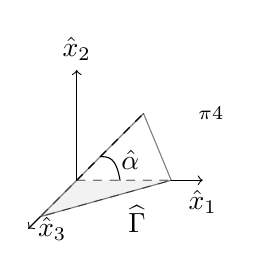
\begin{tikzpicture}[line join = round, line cap = round]
\coordinate [label=left:] (A) at (0,0,0);
\coordinate [label=above right:] (B) at (1.2,0,0);
\coordinate [label=below:] (C) at (0,0,1.2);
\coordinate [label=above right:] (D) at ( 0.848, 0.848, 0);
\draw[->] (1.2, 0,   0) --   (1.6, 0, 0) node[below] {$\hat{x}_1$};
\draw[->] (0,   0,   0) --   (0, 1.4, 0) node[above] {$\hat{x}_2$};
\draw[->] (0,   0,   1.2) -- (0, 0, 1.6) node[right] {$\hat{x}_3$};
\draw (2.0, 1.05) node[anchor=north east] {$\Tref_{\rfrac{\pi}{4}}$};
\draw (1.0, -0.2) node[anchor=north east] {$\widehat{\Gamma}$};
\draw[-, fill=black!10, opacity=.5, dashed] (A)--(B)--(C)--(A);
\draw[-, opacity=.5] (B)--(C);
\draw[-, opacity=.5] (C)--(D);
\draw[-, opacity=.5] (B)--(D);
\draw (0.55,0.0) .. controls (0.5, 0.3) and (0.4, 0.3) .. node[right] {$\hat{\alpha}$}  (0.3,0.3);
\draw[dashed] (A)--(D);
\end{tikzpicture}
}
& \multicolumn{2}{c}{
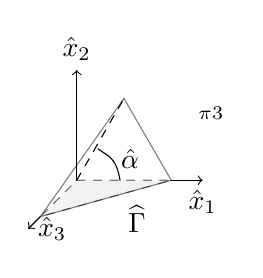
\begin{tikzpicture}[line join = round, line cap = round]
\coordinate [label=left:] (A) at (0,0,0);
\coordinate [label=above right:] (B) at (1.2,0,0);
\coordinate [label=below:] (C) at (0,0,1.2);
\coordinate [label=above right:] (D) at ( 0.6,  1.0392, 0);
\draw[->] (1.2, 0,   0) --   (1.6, 0, 0) node[below] {$\hat{x}_1$};
\draw[->] (0,   0,   0) --   (0, 1.4, 0) node[above] {$\hat{x}_2$};
\draw[->] (0,   0,   1.2) -- (0, 0, 1.6) node[right] {$\hat{x}_3$};
\draw (2.0, 1.05) node[anchor=north east] {$\Tref_{\rfrac{\pi}{3}}$};
\draw (1.0, -0.2) node[anchor=north east] {$\widehat{\Gamma}$};
\draw[-, fill=black!10, opacity=.5, dashed] (A)--(B)--(C)--(A);
\draw[-, opacity=.5] (B)--(C);
\draw[-, opacity=.5] (C)--(D);
\draw[-, opacity=.5] (B)--(D);
\draw (0.55,0.0) .. controls (0.5, 0.3) and (0.4, 0.3) .. node[right] {$\hat{\alpha}$}  (0.27,0.4);
\draw[dashed] (A)--(D);
\end{tikzpicture}
}\\
\midrule
$M(N)$ & $\CPTapproxhatalphahat$ & $\CGTapproxhatalphahat$
& $\CPTapproxhatalphahat$ & $\CGTapproxhatalphahat$\\
%& $\CPTapproxhatalphahat$ & $\CGTapproxhatalphahat$
%& $\CPTapproxhatalphahat$ & $\CGTapproxhatalphahat$\\
\midrule
%7   &  0.32430           & 0.76010       & 0.32599       & 0.65465       & 0.36053       & 0.6547 & 0.41521 &  0.68616 \\
%26  &  0.33854           & 0.82945       & 0.34027       & 0.76128       & 0.37367       & 0.7516 & 0.42748 &  0.86332 \\
%63  &  0.34112           & 0.83133       & 0.34256       & 0.76290       & 0.37559       & 0.7520 & 0.42864 &  0.86460 \\
%124 &  0.34115       & 0.83134       & 0.34259       & 0.76291       & 0.37560       & 0.7520 & 0.42867 &  0.86463 \\
%{\bf 215} &  {\bf 0.34115} & {\bf 0.83134} & {\bf 0.34259} & {\bf 0.76291} & {\bf 0.37560} & {\bf 0.75200} & {\bf 0.42867} &  {\bf 0.86463} \\
7   &  0.32431 & 0.760099 & 0.325985 & 0.654654 \\%& 0.360532 & 0.654654 & 0.4152099 &  0.686161 \\
26  &  0.338539 & 0.829445 & 0.340267 & 0.761278 \\%& 0.373669 & 0.751615 & 0.4274757 &  0.863324 \\
63  &  0.341122 & 0.831325 & 0.342556 & 0.762901 \\%& 0.375590 & 0.751994 & 0.4286444 &  0.864595 \\
124 &  0.341147 & 0.831335 & 0.342589 & 0.762905 \\%& 0.375603 & 0.751999 & 0.4286652 &  0.864630 \\
215 &  {\bf 0.341147} & {\bf 0.831335} & {\bf 0.342589} & {\bf 0.762905} \\%& {\bf 0.375603} & {\bf 0.751999} & {\bf 0.4286652} &  {\bf 0.864630} \\
\midrule
\multicolumn{1}{c|}{$ $}
& \multicolumn{2}{c|}{ $\hat{\theta} = \tfrac{\pi}{2}, \hat{\alpha} = \tfrac{\pi}{2}$}
& \multicolumn{2}{c}{ $\hat{\theta} = \tfrac{\pi}{2}, \hat{\alpha} = \tfrac{2\pi}{3}$}\\
\midrule
\multicolumn{1}{c|}{$ $}
& \multicolumn{2}{c|}{
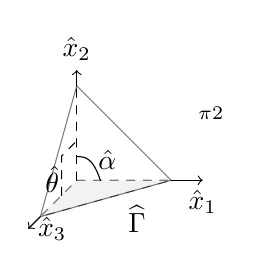
\begin{tikzpicture}[line join = round, line cap = round]
\coordinate [label=left:] (A) at (0,0,0);
\coordinate [label=above right:] (B) at (1.2,0,0);
\coordinate [label=below:] (C) at (0,0,1.2);
\coordinate [label=above right:] (D) at ( 0.0,  1.2, 0);
\draw[->] (1.2, 0,   0) --   (1.6, 0, 0) node[below] {$\hat{x}_1$};
\draw[->] (0,   1.2,   0) --   (0, 1.4, 0) node[above] {$\hat{x}_2$};
\draw[->] (0,   0,   1.2) -- (0, 0, 1.6) node[right] {$\hat{x}_3$};
\draw (2.0, 1.05) node[anchor=north east] {$\Tref_{\rfrac{\pi}{2}}$};
\draw (1.0, -0.2) node[anchor=north east] {$\widehat{\Gamma}$};
\draw[-, fill=black!10, opacity=.5, dashed] (A)--(B)--(C)--(A);
\draw[-, opacity=.5] (B)--(C);
\draw[-, opacity=.5] (C)--(D);
\draw[-, opacity=.5] (B)--(D);
\draw (0.3,0.0) .. controls (0.2, 0.3) and (0.1, 0.3) .. node[right] {$\hat{\alpha}$}  (0.0,0.3);
\draw[dashed] (A)--(D);
\draw[dashed] (0, 0, 0.5)--(0, 0.5, 0.5)--(0, 0.5, 0);
\draw (-0.1, 0.3) node[anchor=north east] {$\hat{\theta}$};

\end{tikzpicture}
} 
& \multicolumn{2}{c}{
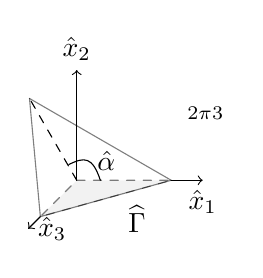
\begin{tikzpicture}[line join = round, line cap = round]
\coordinate [label=left:] (A) at (0,0,0);
\coordinate [label=above right:] (B) at (1.2,0,0);
\coordinate [label=below:] (C) at (0,0,1.2);
\coordinate [label=above right:] (D) at ( -0.6,  1.0392, 0);
\draw[->] (1.2, 0,   0) --   (1.6, 0, 0) node[below] {$\hat{x}_1$};
\draw[->] (0,   0,   0) --   (0, 1.4, 0) node[above] {$\hat{x}_2$};
\draw[->] (0,   0,   1.2) -- (0, 0, 1.6) node[right] {$\hat{x}_3$};
\draw (2.0, 1.05) node[anchor=north east] {$\Tref_{\rfrac{2\pi}{3}}$};
\draw (1.0, -0.2) node[anchor=north east] {$\widehat{\Gamma}$};
\draw[-, fill=black!10, opacity=.5, dashed] (A)--(B)--(C)--(A);
\draw[-, opacity=.5] (B)--(C);
\draw[-, opacity=.5] (C)--(D);
\draw[-, opacity=.5] (B)--(D);
\draw (0.3,0.0) .. controls (0.2, 0.3) and (0.1, 0.3) .. node[right] {$\hat{\alpha}$}  (-0.1,0.2);
\draw[dashed] (A)--(D);
\end{tikzpicture}
}\\
\midrule
$M(N)$ & $\CPTapproxhatalphahat$ & $\CGTapproxhatalphahat$
& $\CPTapproxhatalphahat$ & $\CGTapproxhatalphahat$\\
\midrule
7   & 0.360532 & 0.654654 & 0.4152099 &  0.686161 \\
26  & 0.373669 & 0.751615 & 0.4274757 &  0.863324 \\
63  & 0.375590 & 0.751994 & 0.4286444 &  0.864595 \\
124 & 0.375603 & 0.751999 & 0.4286652 &  0.864630 \\
215 & {\bf 0.375603} & {\bf 0.751999} & {\bf 0.4286652} &  {\bf 0.864630} \\
\midrule
\end{tabular}
\caption{$\CPTapproxhatalphahat$ and $\CGTapproxhatalphahat$ with
respect to $M(N)$ for $\Tref_{\hat{\theta}, \hat{\alpha}}$ with 
$\rho = 1$, $\hat{\theta} = \tfrac{\pi}{2}$, and several $\hat{\alpha}$.}
\label{tab:const-convergence-from-basis-G-leg-alpha}
\end{table}

To the best of our knowledge, exact values of constants in Poincar\'{e}-type 
inequalities for simplexes in $\Rthree$ are unknown. Therefore, in  
\cite{RefArxivMatculevichRepin2015} some reference cases are calculated numerically with high accuracy and listed in Table \ref{tab:const-convergence-from-basis-G-leg-alpha}. 
%
Based on these data, we present the (approximate) bounds for an arbitrary tetrahedron $\T$:
%
\begin{alignat}{2}
    \|v\|_{\T} \, & \leq\, \CPtetr \, h_1 \, h_3 \,\|\nabla v\|_{\T}, \qquad \; \;
    \CPtetr = 
		\min_{\hat{\alpha} = \{\rfrac{\pi}{4}, \rfrac{\pi}{3}, \rfrac{\pi}{2}, \rfrac{2\pi}{3}\}} 
		\Big\{ \cpalphahat \, \CPThatalphahat \Big\},\nonumber \\
    %
    \|v\|_\Gamma \, & \leq\, \CGtetr    \,
    (h_1 \, h_3)^{\footnotesize \tfrac{1}{2}} \,\|\nabla v\|_{\T}, \quad
   	\CGtetr = 
		\min_{\hat{\alpha} = \{\rfrac{\pi}{4}, \rfrac{\pi}{3}, \rfrac{\pi}{2}, \rfrac{2\pi}{3}\}} 
		\Big\{ \cgalphahat \, \CGThatalphahat \Big\},
		\label{eq:general-poincare-type-inequalities-for-tetrahedron}
\end{alignat}
%
where $\CPThatalphahat$ and $\CGThatalphahat $ are the constants related to four reference thetrahedron from Table \ref{tab:const-convergence-from-basis-G-leg-alpha} and 
%
\begin{equation*}
  \cpalphahat = \tfrac{\mu^{\rfrac{1}{2}}_{\pi/2, \hat{\alpha}}}{h_1 h_3}, \quad
  \cgalphahat = 
	\Big(  \tfrac{h_3 \sin \hat{\alpha}}{\rho \sin\alpha \sin\theta}\Big)^{\rfrac{1}{2}} \,\cpalphahat.
\end{equation*}
%
are the ratios of the mapping 
$\mathcal{F}_{\rfrac{\pi}{2}, \hat{\alpha}}$: 
$\Tref_{\rfrac{\pi}{2}, \hat{\alpha}} \rightarrow \T$. Here, \linebreak
$\Tref_{\rfrac{\pi}{2}, \hat{\alpha}} :=
 {\rm conv} \big \{(0, 0, 0), (1, 0, 0), (0, 0, 1), 
(\cos\hat{\alpha}, \sin\hat{\alpha}, 0) \big\}$ with 
$\hat{\alpha} = 
\{ \tfrac{\pi}{4}, \tfrac{\pi}{3}, \tfrac{\pi}{2}, \tfrac{2\pi}{3}\}$,
$\T$ is defined in (\ref{eq:arbitrary-tetrahedron}), and 
$\mathcal{F}_{\rfrac{\pi}{2}, \hat{\alpha}}(\hat{x})$ is presented by the relation
%
\begin{equation*}
    x = \mathcal{F}_{\rfrac{\pi}{2}, \hat{\alpha}}(\hat{x}) =
    B_{\rfrac{\pi}{2}, \hat{\alpha}} \hat{x}, \quad
    B_{\rfrac{\pi}{2}, \hat{\alpha}} =
    \begin{pmatrix}
        \: h_1 & 
				\; \tfrac{h_1}{\sin \hat{\alpha}} 
				   (\rho \cos\alpha \sin\theta - \cos \hat{\alpha}) & 
				\; 0 \\[0.3em]
        \: 0 & 
				\; h_1 \rho \tfrac{\sin\alpha \sin(\theta)}{\sin \hat{\alpha}} \: & 
				\: 0 \\[0.3em]
        \: 0 & 
				\; h_1 \rho \tfrac{\cos\theta}{\sin \hat{\alpha}} \: & 
				\: h_3 \\
    \end{pmatrix}.
	%\label{eq:3d-mapping}
\end{equation*}
%
%

The numerical tests and detailed 
discussions of the practical aspects of this study can be found in
\cite{RefArxivMatculevichRepin2015}. In \cite[Section 5]{RefArxivMatculevichRepin2015},
we provide an example that shows possible applications of the results and derive a 
computable majorant of the difference between the exact solution of a boundary value 
problem and an arbitrary finite dimensional approximation computed on a simplicial mesh.
Using the above presented constants, one can weaken the pointwise continuity condition 
of normal components of the auxiliary flux on inner faces of the mesh in the functional 
estimates \eqref{eq:majorant-decomposed-I}. Instead, it is enough that the mean values of 
the normal components are continuous, which allows us to use a wider space for the 
approximation of the flux. 



